In this section, we subject the JP structures to various
background flows. The purpose is to understand how the self-assemblies
respond to external forcing. We then compare effective
properties of materials comprised of JPs as a function of
their amphiphilic properties.
%%%

\subsection{Bilayer configurations (BC (i)) in a linear shear flow}
To begin, we place the bilayer structure (with BC (i)) from the inset of
Figure~\ref{fig:relax}(b) in a linear shear flow
\begin{equation}
\uu_\infty(\xx) = \dot\gamma \text{ ns }^{-1} ({\bf e}_y \cdot \mathbf{x}) {\bf e}_x,
\end{equation}
%
where $\dot\gamma$ is the dimensionless shear rate, and ${\ee}_x$ and
${\ee}_y$ are horizontal and vertical unit vectors, respectively. The
initial bilayer structure consists of a small self-enclosing bilayer
(vesicle) and several pieces of bilayers.
Figure~\ref{fig:BC1_shear}(a)--(c) shows a snapshot at $t = 0.5$
$\upmu$s of the bilayer for different shear rates $\dot\gamma=
0.05,0.075,0.01$. The dynamics of the bilayer can be found in
Supplementary Movie S2, which shows
that the initial pieces of bilayers
merge and form a worm-like shape under a linear shear flow. At a low
shear rate, the bilayer constantly goes through rotation and extensional
deformation with the whole bilayer remaining intact
(Figure~\ref{fig:BC1_shear}(a)). As the shear rate increases to a
moderate value (Figure~\ref{fig:BC1_shear}(b)), the bilayer is observed
to shed a small piece of bilayer, similar to the asymmetric breakup of a
viscous drop in confinement \cite{DuFuZhuMaLi2016_AICHEJ}.
%\todo[inline]{missing citation}. 
In Figure~\ref{fig:BC1_shear}(c) the high shear rate gives rise to two
separate, nearly equal bilayers, similar to the symmetric drop breakup
under a linear shear flow \cite{Stone1994_ARFM}. For the dynamic evolution, see
Supplementary Movie S4.

%\todo[inline]{missing citation}.
%%
%\begin{figure}
%  \begin{center}
%    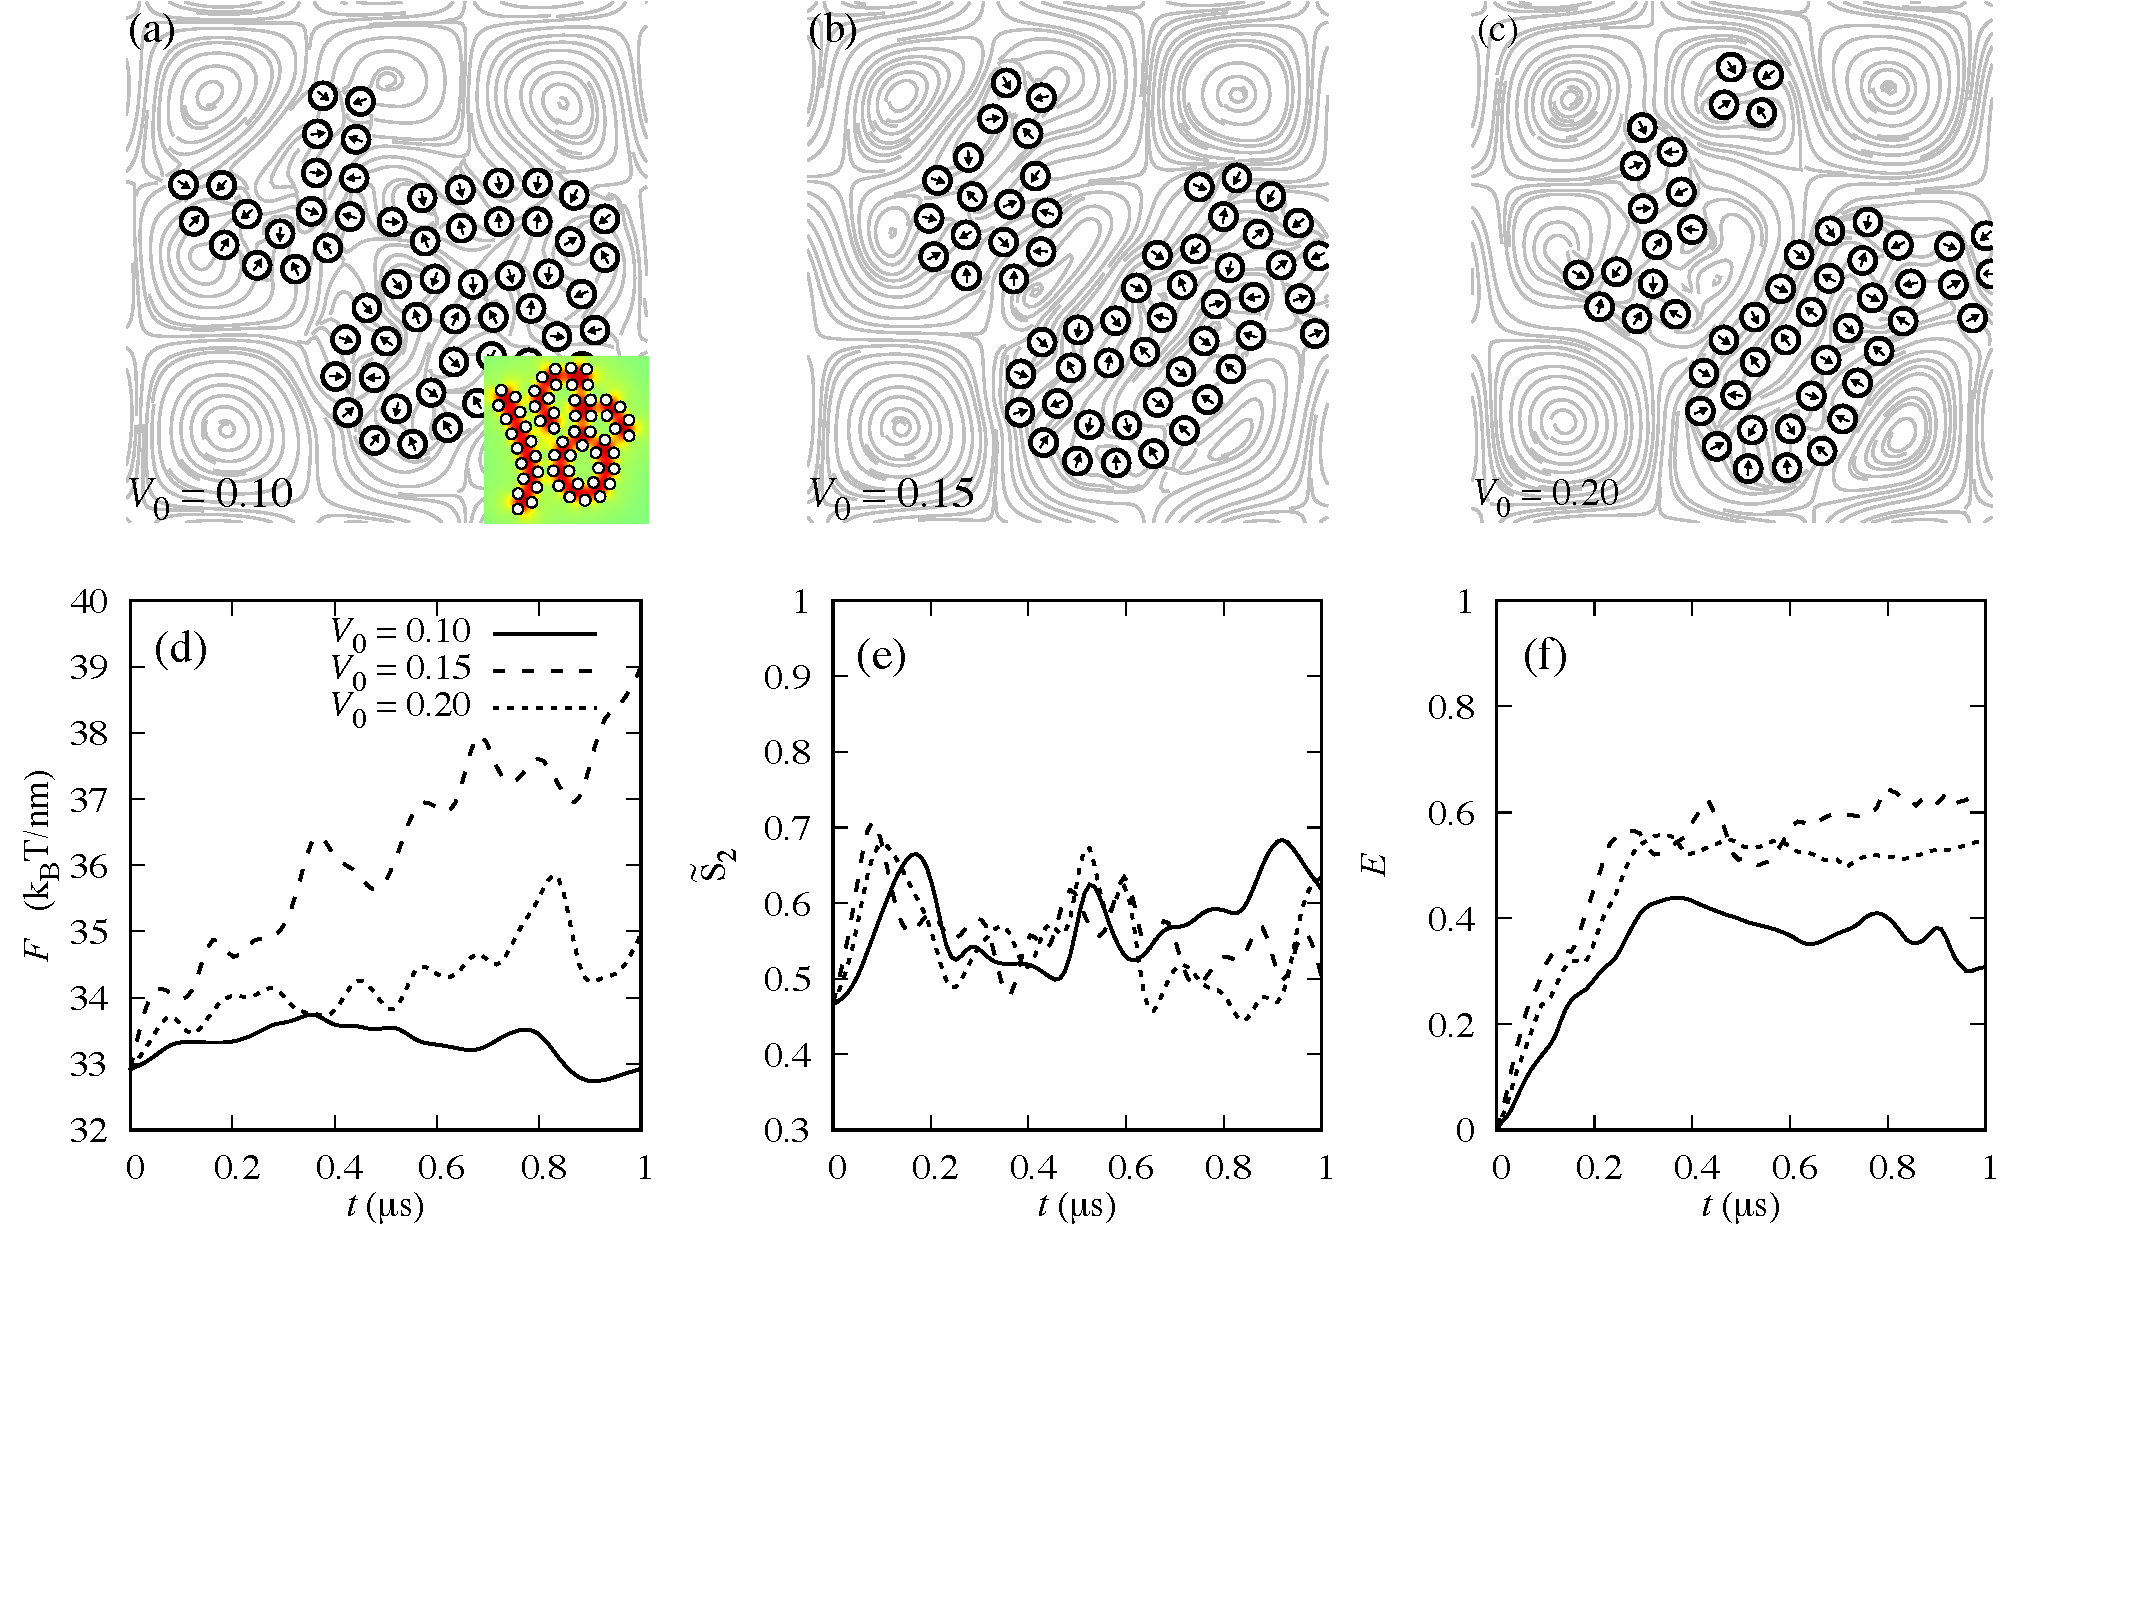
\includegraphics[width=1.0\textwidth]{Figures/Figure5.pdf}    
%  \end{center}
%  \vspace{-20pt}  
%  \caption{\label{fig:BC1_TG} Multiple component bilayers in a Taylor-Green when $V_0 = \{0.1, 0.15, 0.2\}$ at $t=0.2\ \mu$s. The pre-relaxed initial configuration is shown in inset of panel (a). 
% The streamlines are plotted in the background. 
%Panel (d) plots the free energies; panel (e) shows orientational parameter $\tilde{S}_2$; panel (f) shows positional parameter E.
%  }
%\end{figure}

We observe that the order parameter $\tilde S_2$ in
Figure~\ref{fig:BC1_shear}(e) is on average increasing. In the initial
configuration, the structure has three or four pieces of bilayer.
%
Under the shear flow, the shedding and merging of bilayers results in an
overall decrease in distinct bilayer structures. Similarly, the free
energies are slightly decreasing (Figure~\ref{fig:BC1_shear}(d)), with
the overall changes occurring in the range of a few $\mathrm{k_BT}$/nm.
This suggests that the shear flow changes the energy landscape to move
the local equilibrium obtained from a random initial condition to an
alternate local equilibrium with less free energy and greater
orientational order  (Supplementary Movie S2).  Note that the free energy $F$ in
Figure~\ref{fig:BC1_shear}(d) has the unit of force ($\mathrm{k_BT}$/nm $\approx$ 4.114 pN)
because our system
is two dimensional.
%
%\begin{figure}
%  \begin{center}
%    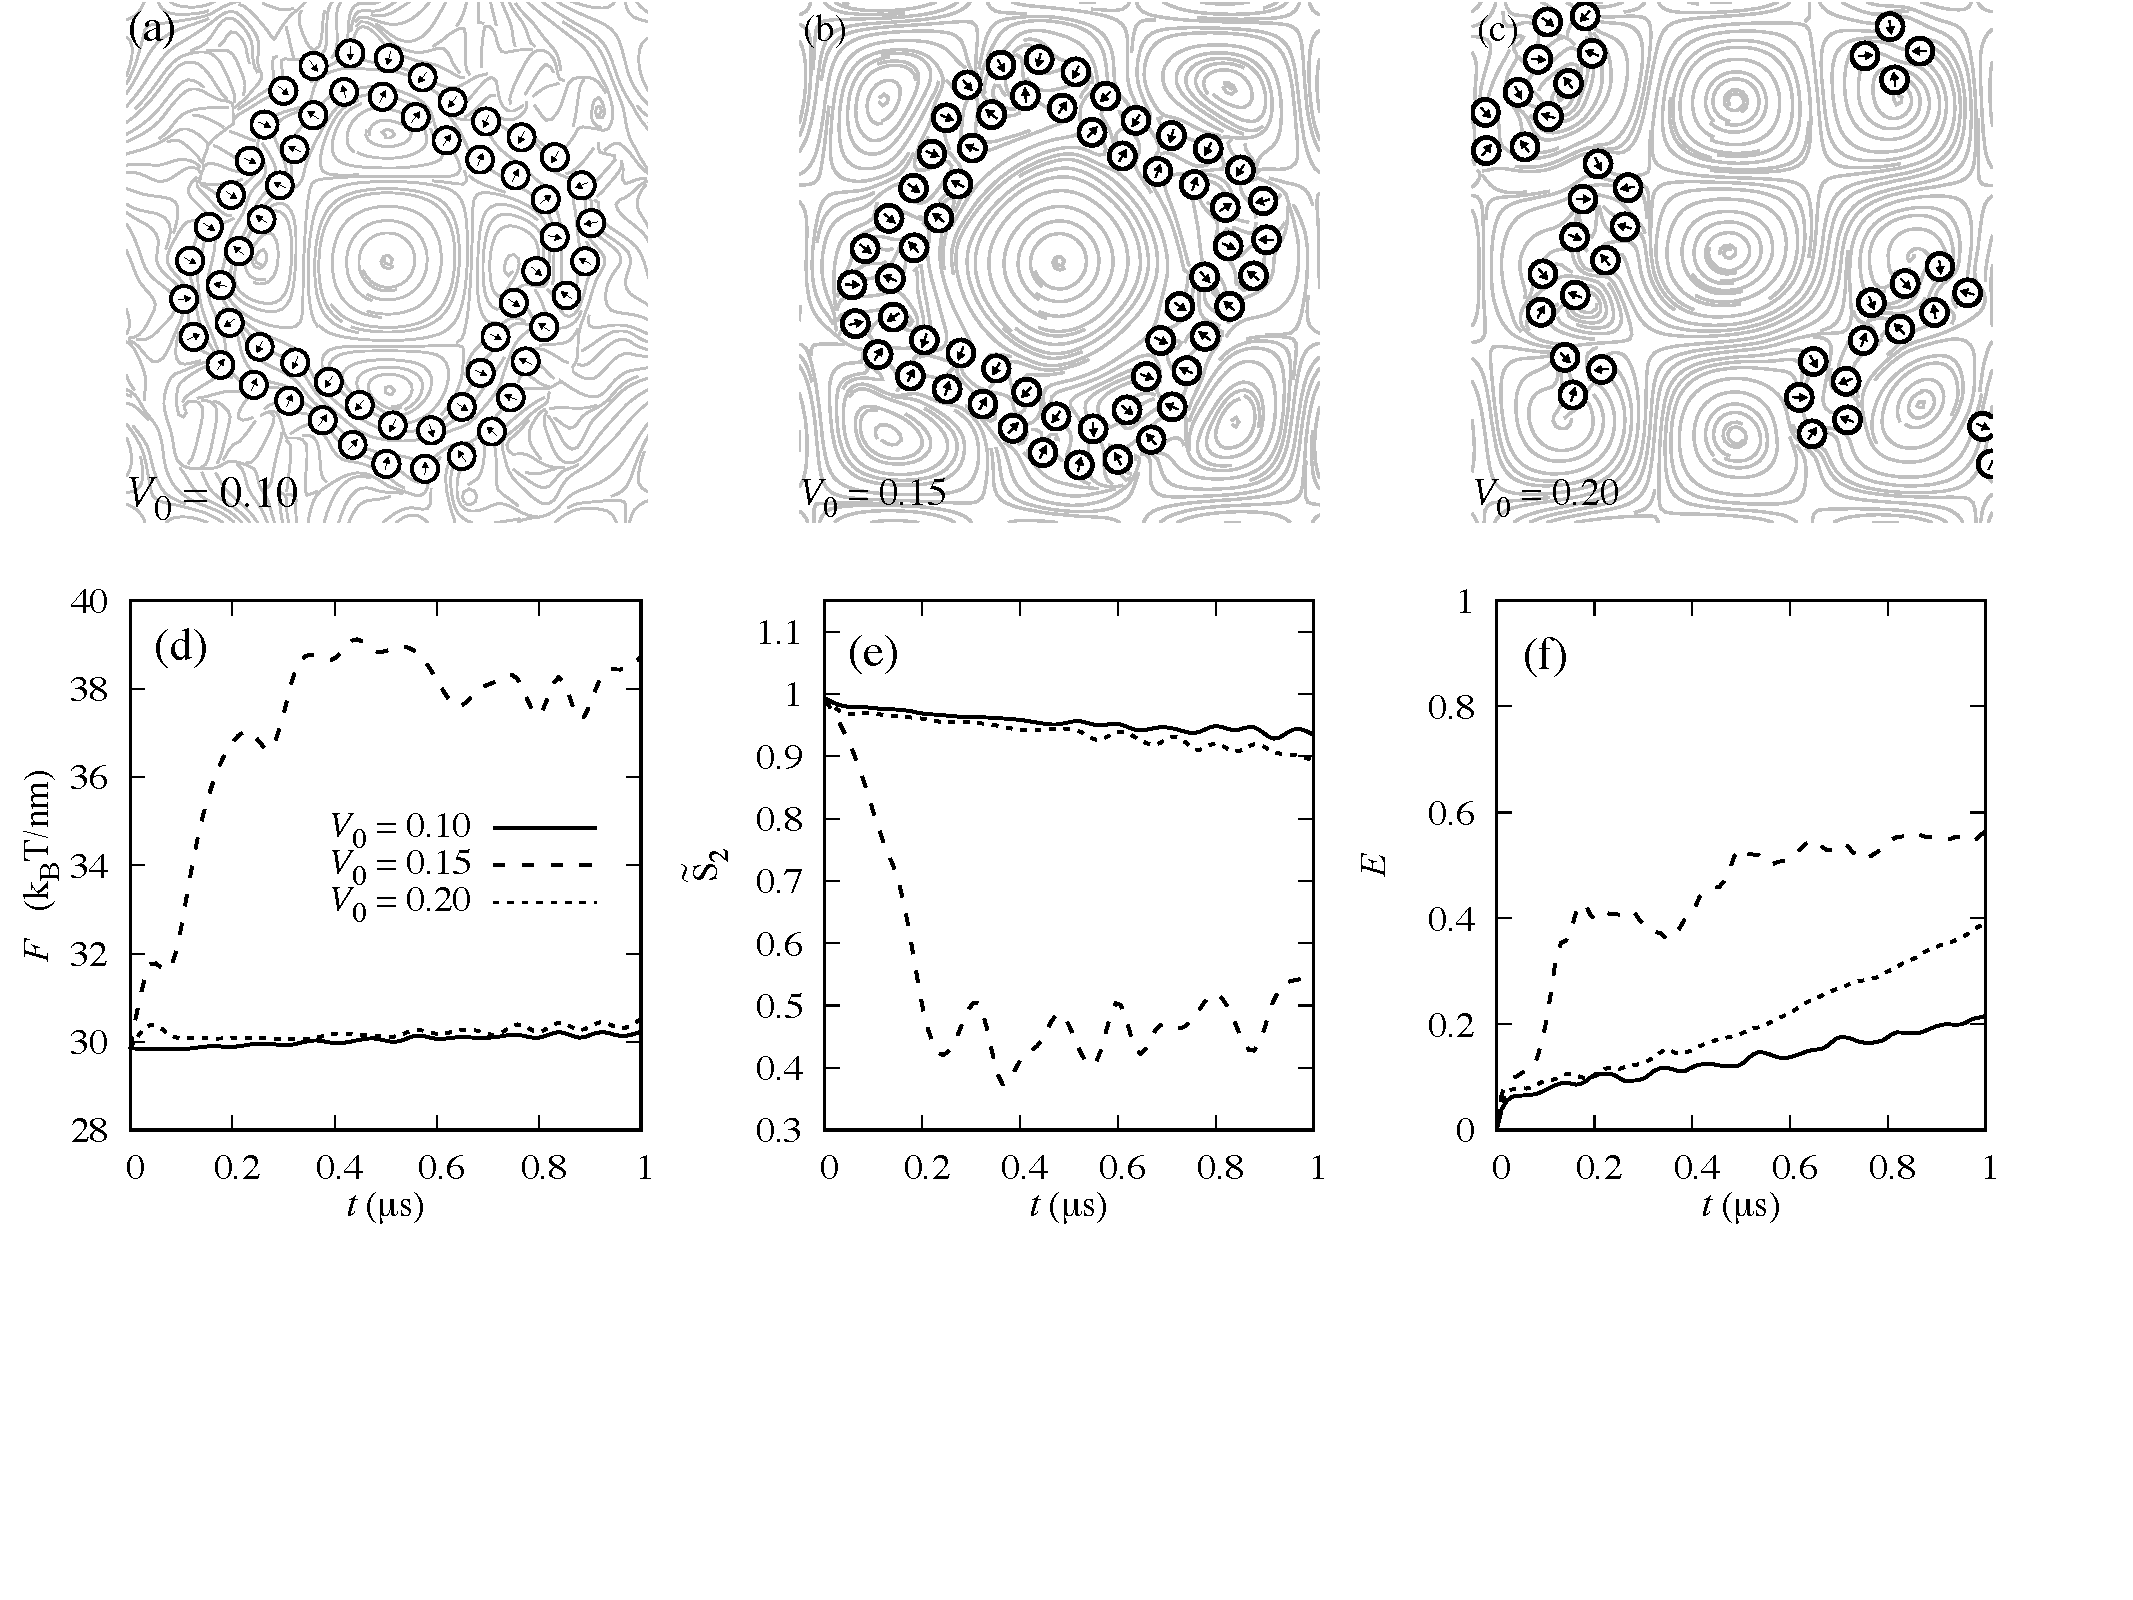
\includegraphics[width=1.0\textwidth]{Figures/Figure6.pdf}        
%  \end{center}
%\caption{\label{fig:ves_TG} Single vesicle in a TG flow. Panels (a)-(c) are snapshots for $V_0=\{0.1, 0.15, 0.2\}$ at $t=0.6\ \mu$s where the pre-relaxed initial configuration is shown in inset of panel (a). The streamlines are plotted in the background.
%Panel (d) plots the free energies; panel (e) shows orientational parameter $\tilde{S}_2$; panel (f) shows positional parameter E.
%}
%\end{figure}
%
Finally, the strain parameter diverges in the large shear rate cases
(Figure~\ref{fig:BC1_shear}(f))
because the various pieces of bilayer eventually completely separate and move away from one another
under the shear flow.

%%%
\begin{figure}
  \begin{center}
    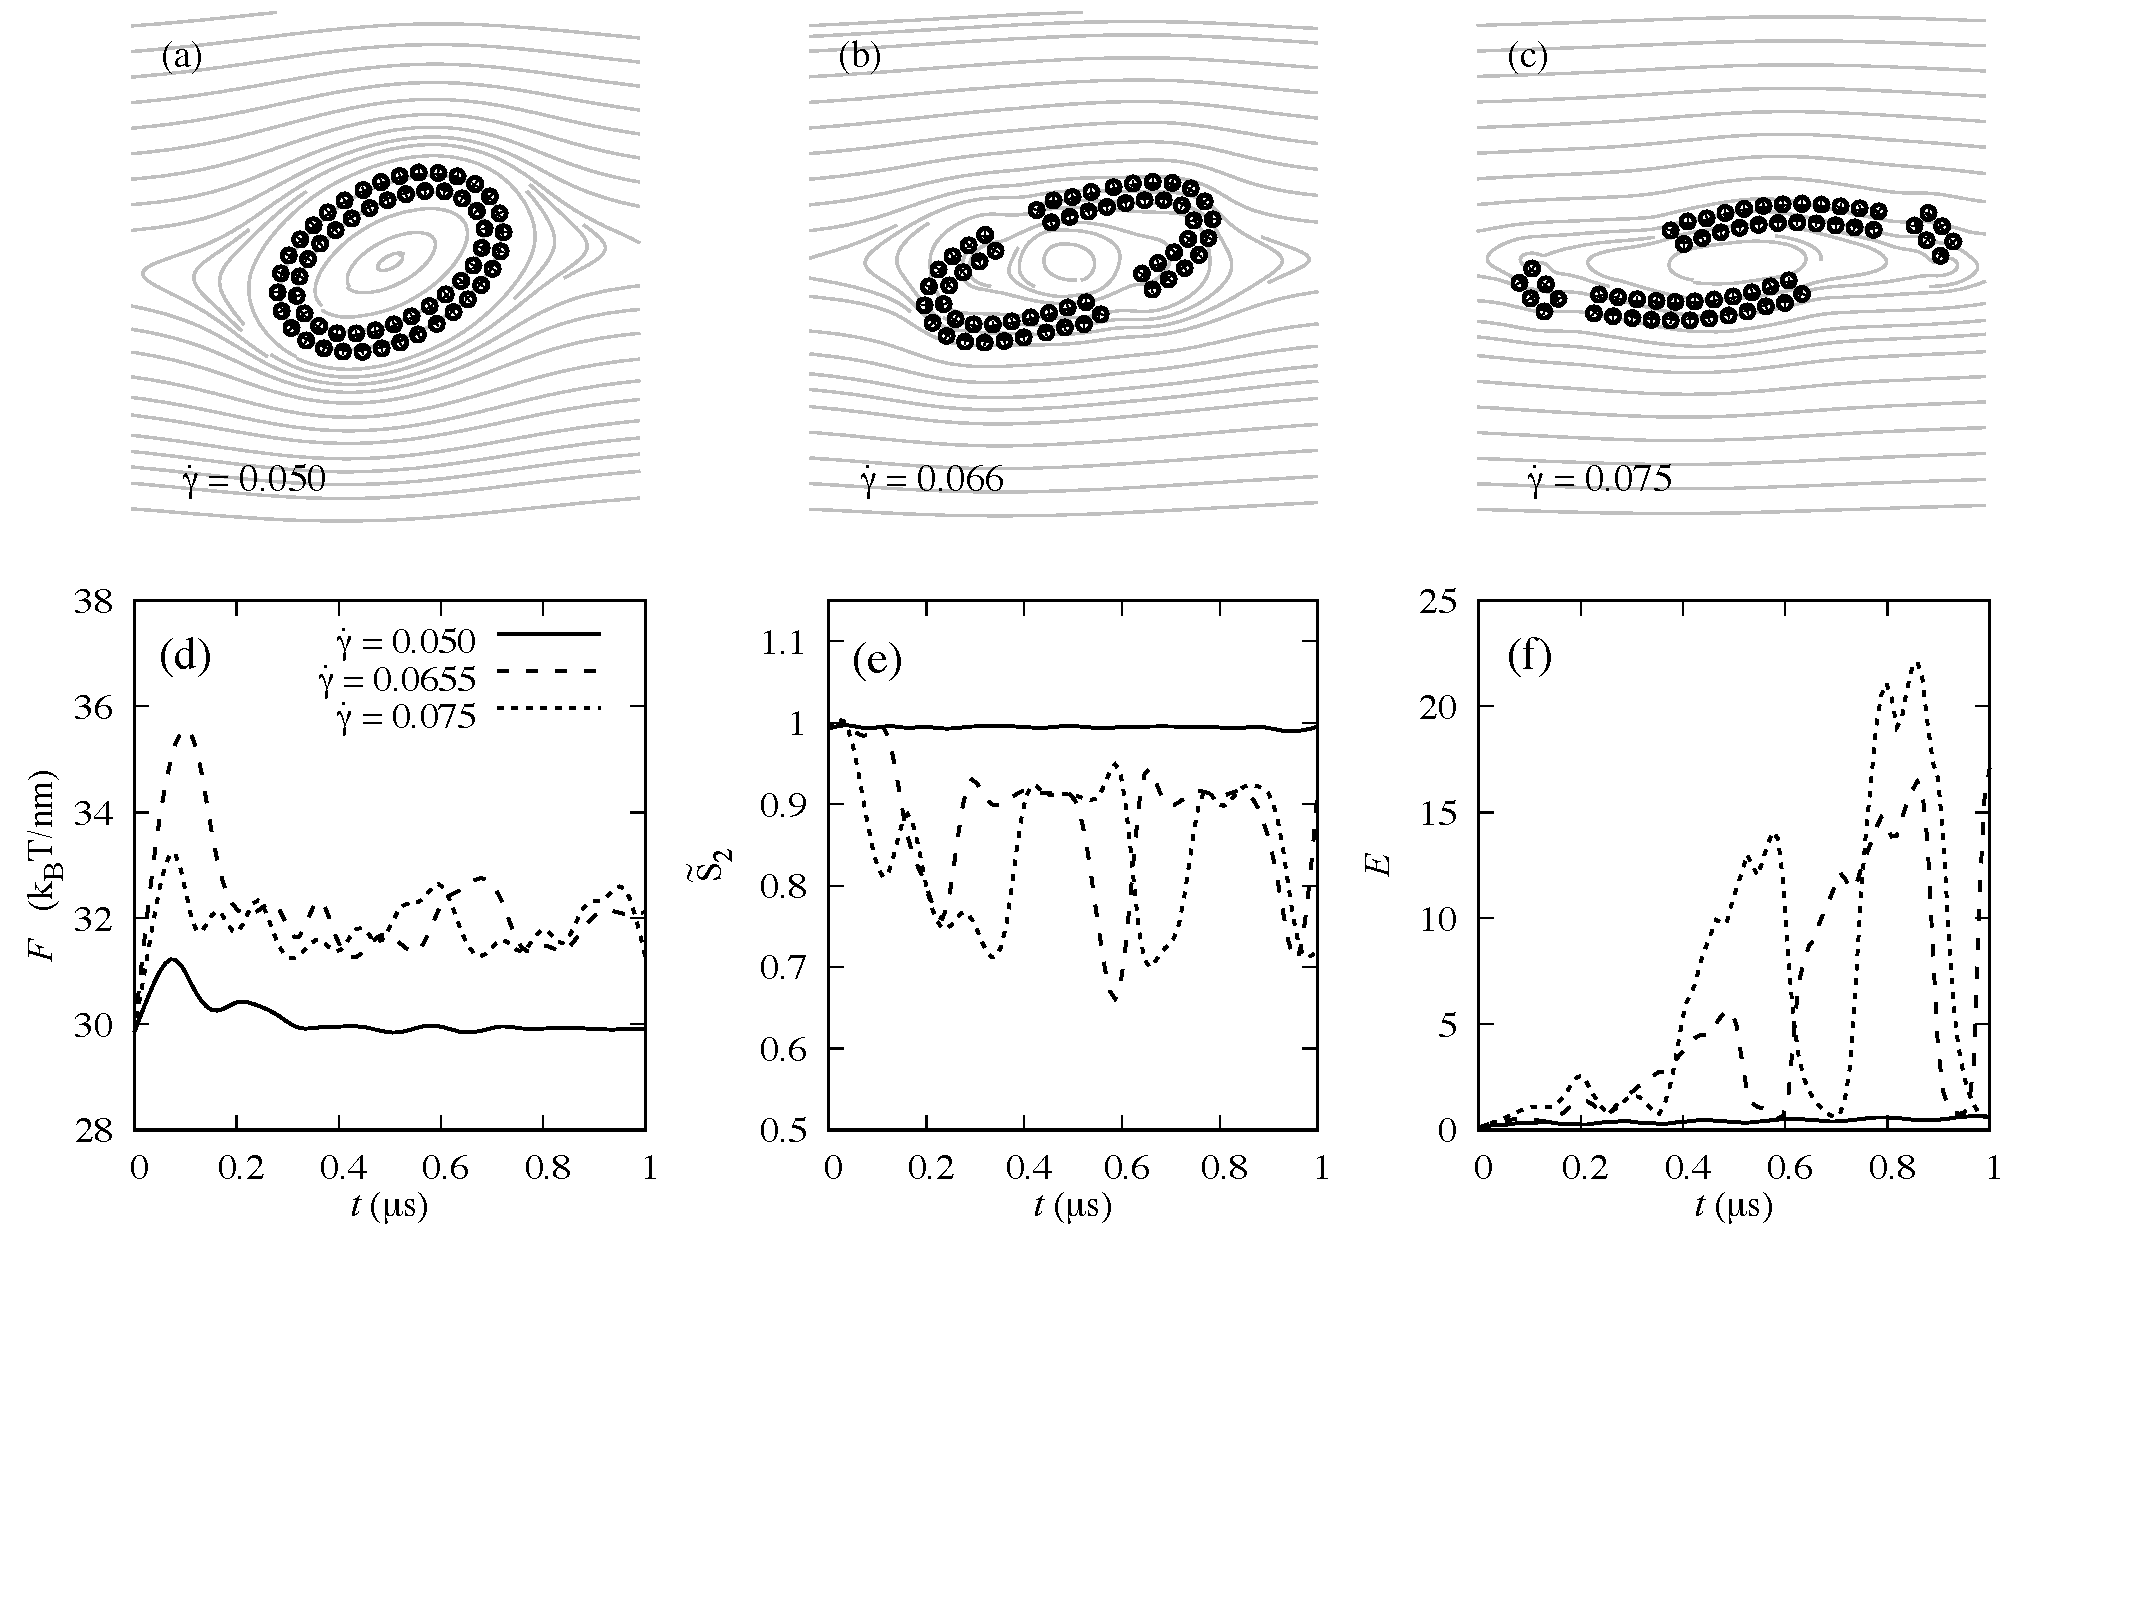
\includegraphics[width=1.0\textwidth]{Figures/Figure4.pdf}
  \end{center}
  \caption{
    \label{fig:Ves_shear}
A single vesicle in a shear flow. Panels (a)--(c) are snapshots for
  $\dot \gamma = \{0.05, 0.0655, 0.075\}$ at $t=0.16\ \upmu$s where the
  pre-relaxed initial configuration is shown in inset of panel (a). The
  streamlines are plotted in the background. Panel (d) shows the free
  energies; panel (e) shows orientational parameter $\tilde{S}_2$; panel
  (f) shows positional parameter E.}
\end{figure}
\citet{Fu2022_JFM} studied the hydrodynamics of a JP vesicle under a
linear shear flow. Focusing on drawing analogies to hydrodynamics of a
vesicle in continuum modeling (such as
tank-treading~\cite{keller_skalak_1982,Finken08,Shaqfeh11}, bilayer
slip~\cite{sch-vla-mik2010,denOtter2007,Zgorski2019}, and
permeability~\cite{chabanon2017, qua-gan-you2021}), our previous work
demonstrated the existence of a critical shear rate above which the JP vesicle
ruptures~\cite{grandmaison_brancherie_salsac_2021,D2SM00179A}. Based on
the these early results, we reinitialized the BC (i) configuration in
the form of a single, circular vesicle (rather than several bilayer
components) and illustrate how the three measures of structural
deformation correlate to the dynamics of a JP vesicle.

At shear rates $\dot\gamma=0.05, 0.066, 0.075$, the vesicle undergoes
familiar hydrodynamics, such as elongation along the extensional axis
and tank-treading motion, as shown in
Figure~\ref{fig:Ves_shear}(a)--(c)
and Supplementary Movie S2.
%
The circular shape is also a local equilibrium, with somewhat less
energy than the disordered state c.f., Figure~\ref{fig:BC1_shear}(d) and
Figure~\ref{fig:Ves_shear}(d). But unlike the dynamics of bilayers in
Figure~\ref{fig:BC1_shear}, the energies of the JP vesicle in
Figure~\ref{fig:Ves_shear}(d) jump from the baseline value 30
$\mathrm{k_BT}$/nm to about 32 $\mathrm{k_BT}$/nm, signaling the rupture
of the vesicle into disconnected bilayers (see
Figure~\ref{fig:Ves_shear}(d), long and short dashed curves).  After the
rupture, each piece circles around the vorticity at the center without
reconnection while the energies fluctuate slightly around a constant.

For the lowest shear rate case, the vesicle has nearly constant
orientational order $\tilde S_2 = 1$ (see Figure~\ref{fig:Ves_shear}(e),
solid curve). After the JP vesicle ruptures with $\dot\gamma= 0.066$ and
$\dot \gamma= 0.075$, we observe a greater variation in the order
parameter $\tilde{S}_2$ with a baseline value around $0.7$ (see
Figure~\ref{fig:Ves_shear}(e), dashed curves). The oscillations occur
due to the orbit of the two bilayer components, and $\tilde{S}_2$
increases to about $0.9$ when the components slide past one another and
are nearly parallel.
%
As in the previous case, peaks in the strain parameter $E$ correlate
well with changes in structural topology in the bilayer dynamics (dashed
curves in Figure~\ref{fig:Ves_shear}(f)).


%%%%%%%
%
\begin{figure}
  \begin{center}
    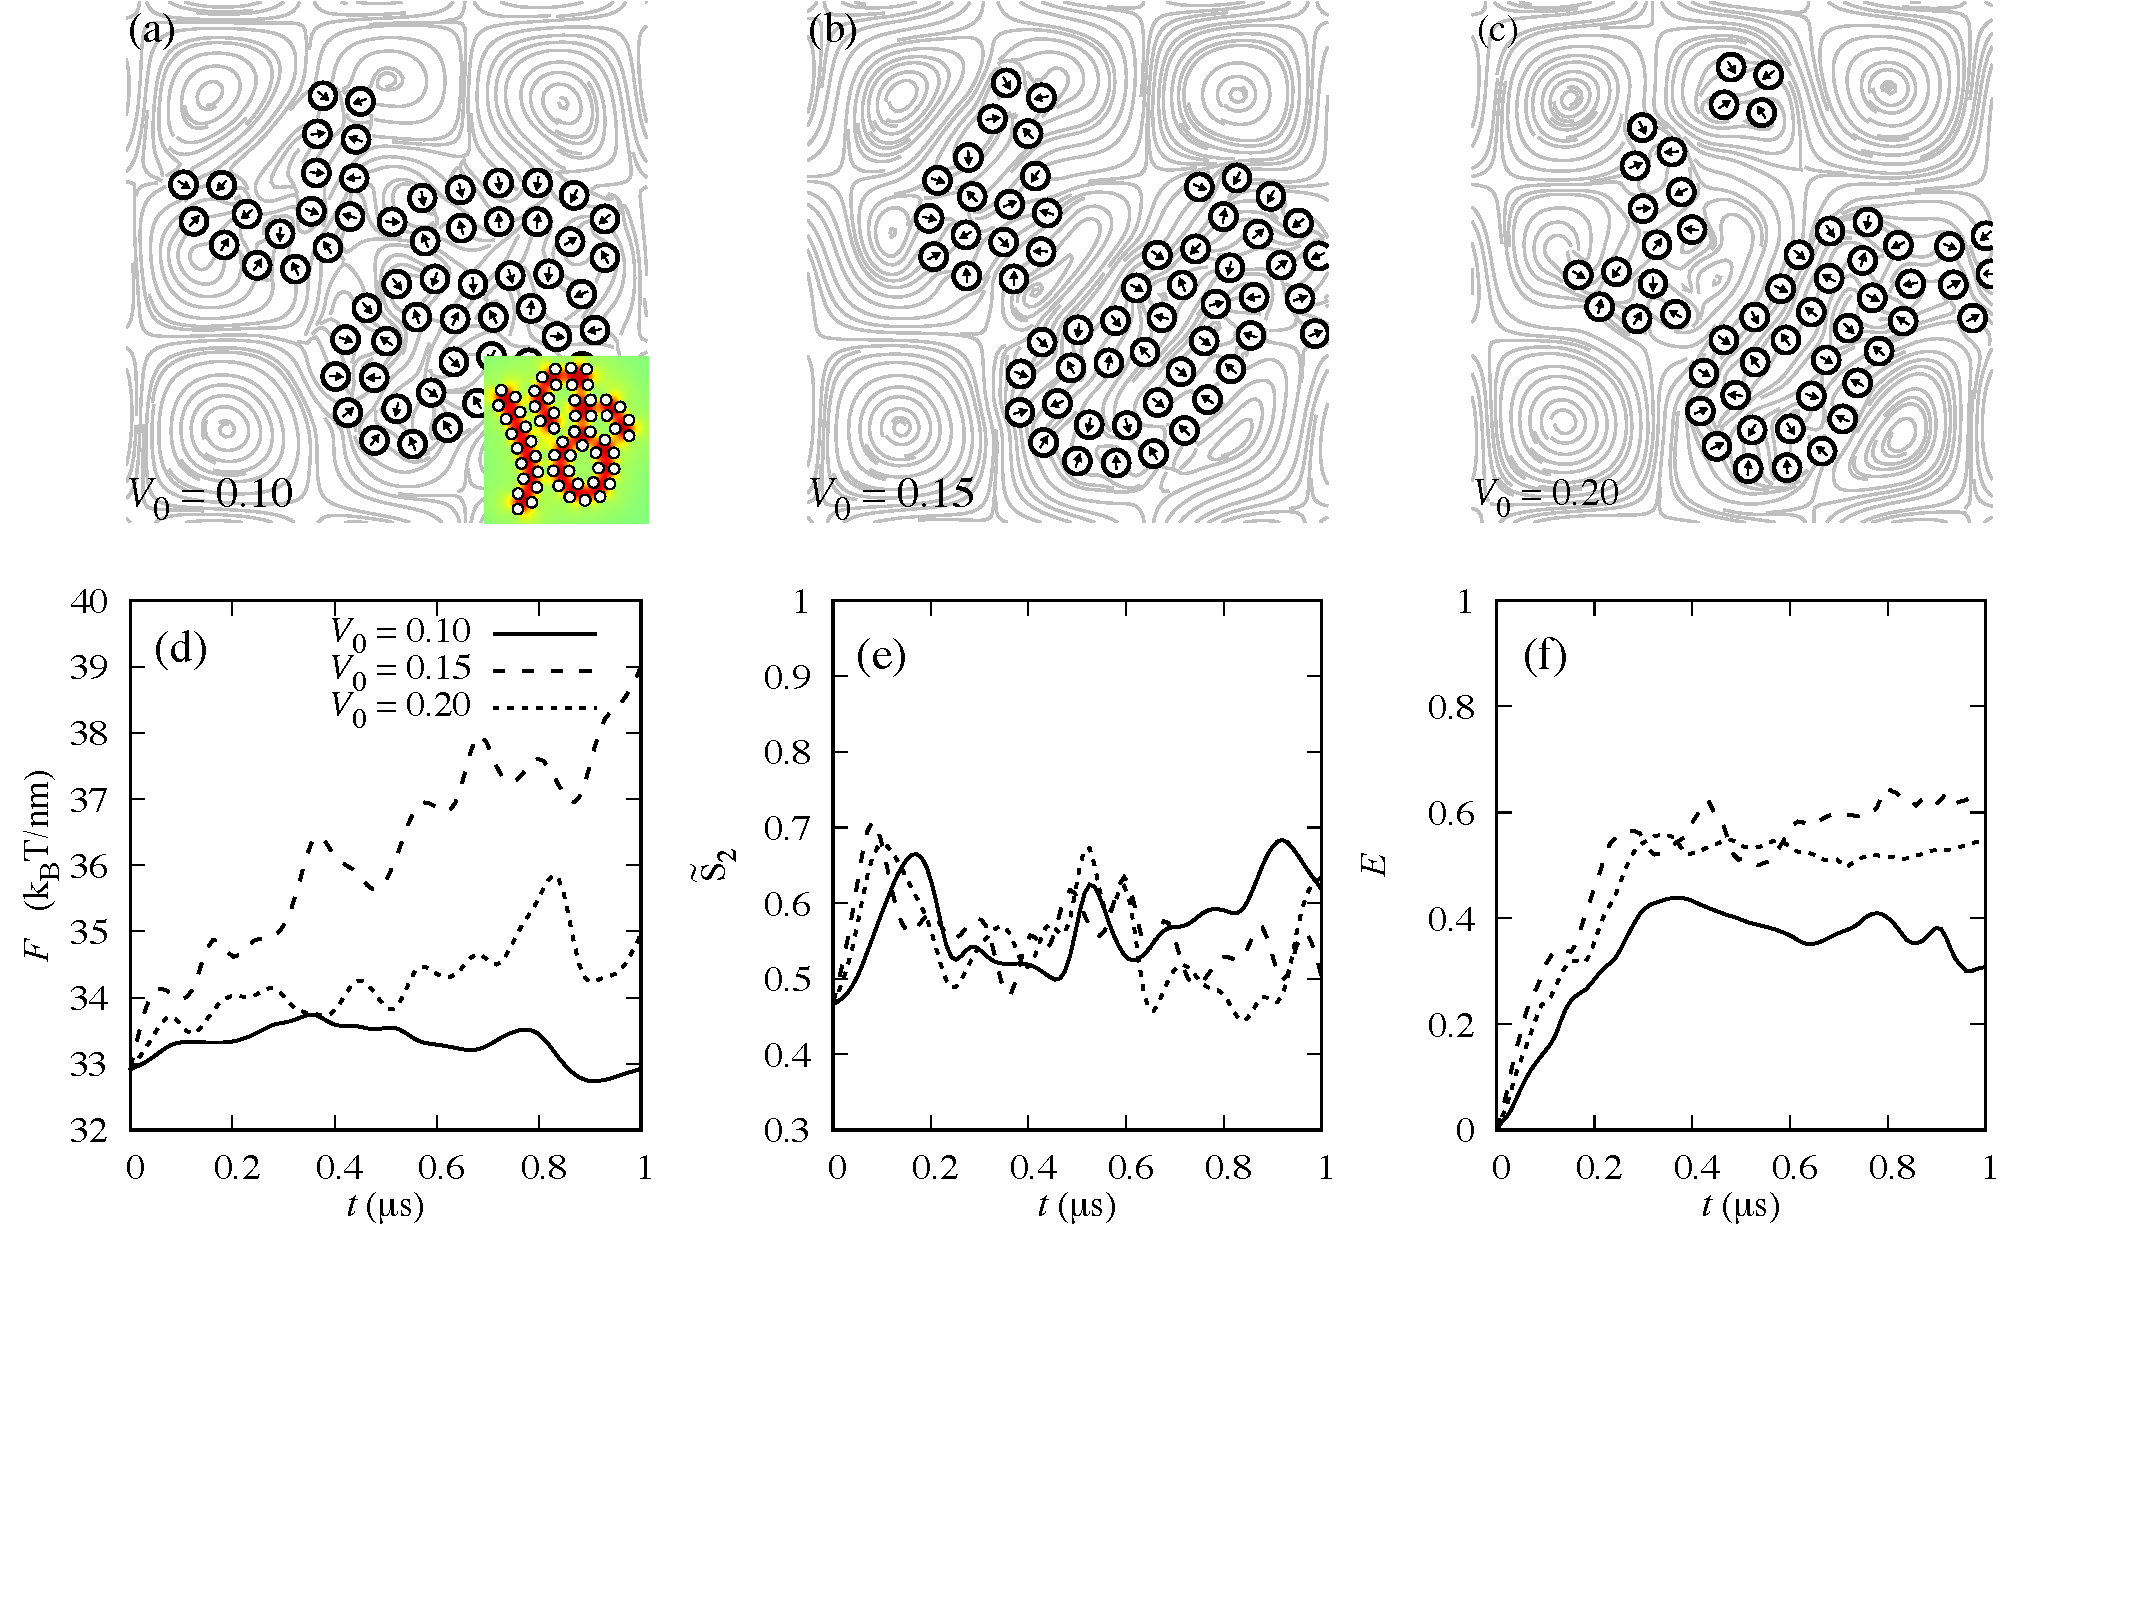
\includegraphics[width=1.0\textwidth]{Figures/Figure5.pdf}    
  \end{center}
  \vspace{-20pt}  
  \caption{\label{fig:BC1_TG} Bilayers with multiple domains in a
  Taylor-Green when $V_0 = \{0.1, 0.15, 0.2\}$ at $t=0.2\ \upmu$s. The
  pre-relaxed initial configuration is shown in the inset of panel (a).
  The streamlines are plotted in the background. Panel (d) shows the
  free energies; panel (e) shows the orientational parameter
  $\tilde{S}_2$; panel (f) shows the positional parameter $E$.}
\end{figure}
%
\subsection{Bilayer and vesicle configurations in a Taylor-Green flow}
Next, we subject the JP structures to a steady Taylor-Green (TG) background
flow
\begin{equation}
\label{eq:tg_flow}
\uu_\infty(\xx) = V_0\; \frac{\text{nm}}{\text{ns}}\;
\left(
-\cos\left(x/\lambda\right)
 \sin\left(y/\lambda\right)
         {\bf e}_x
         +\sin\left(x/\lambda\right)
         \cos\left(y/\lambda\right)
             {\bf e}_y\right),
\end{equation}
where $x = {\bf e}_x \cdot \xx$ and $y = {\bf e}_y \cdot \xx$
are the horizontal and vertical coordinates, respectively. 
The TG flow is a confining flow consisting of a checkerboard pattern
of cells with alternating circulation. We control the flow by the
dimensionless flow strength $V_0$ and the dimensionless cell size $l$
defining $\lambda = l$ nm. For most of the results in this subsection,
we use the parameter $l=2$.
%

\begin{figure}
  \begin{center}
    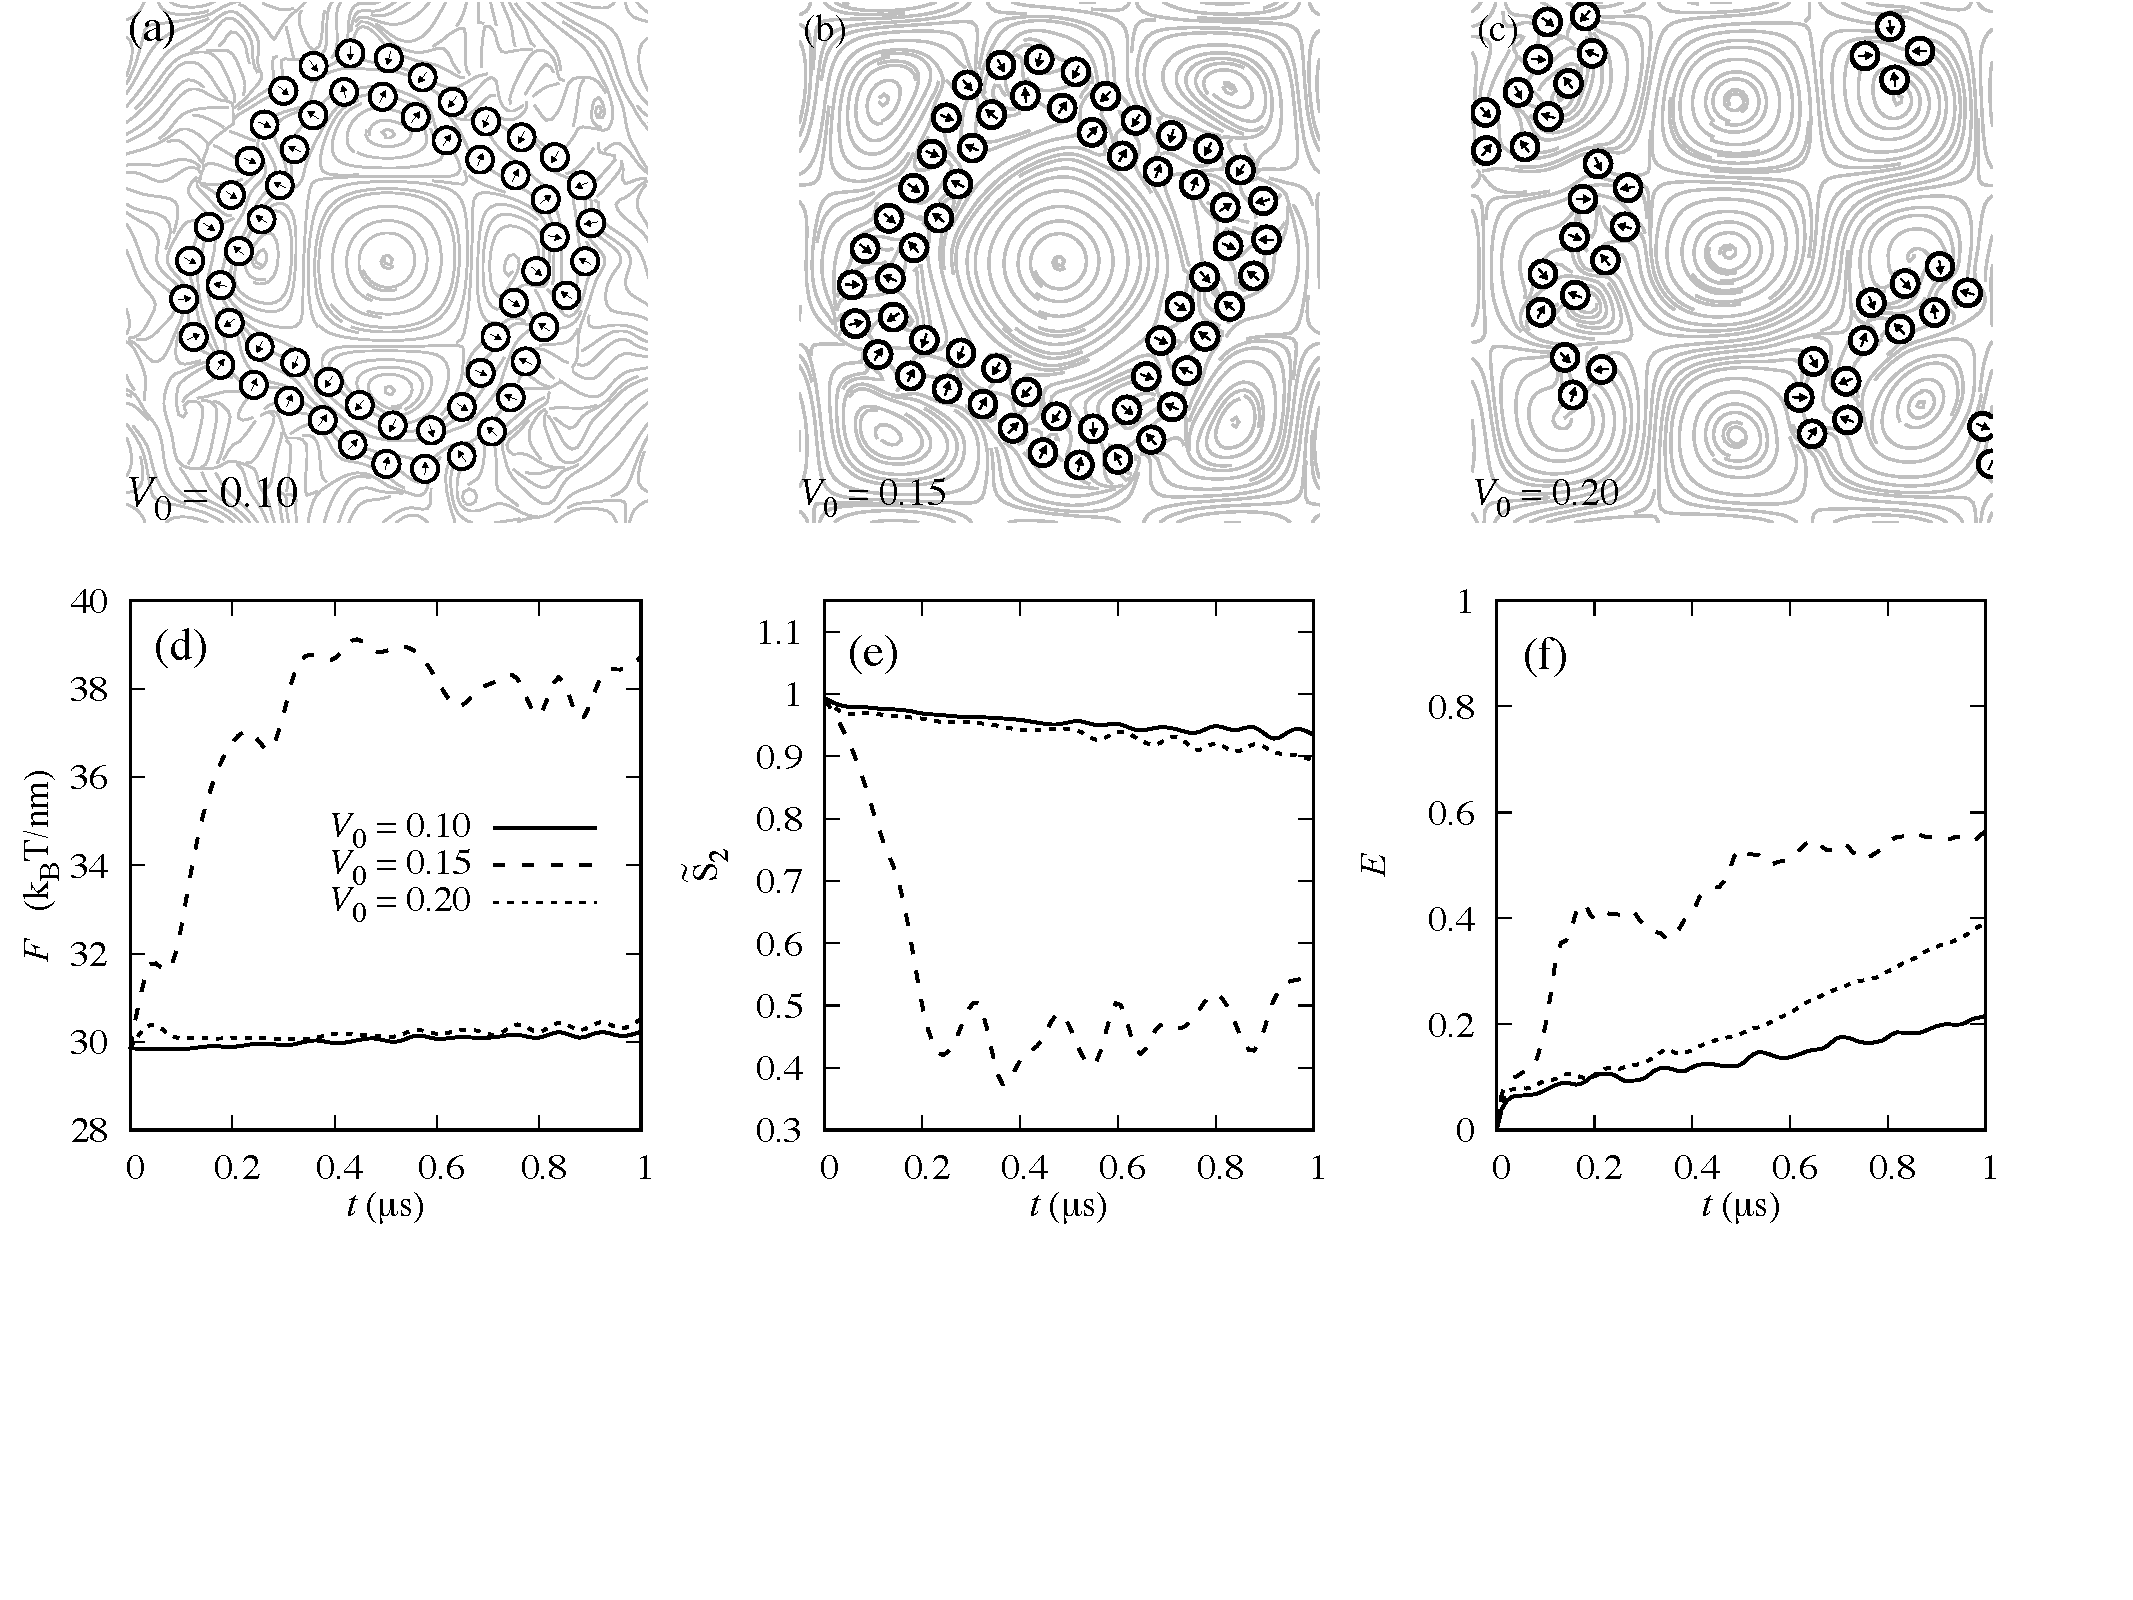
\includegraphics[width=1.0\textwidth]{Figures/Figure6.pdf}        
  \end{center}
\caption{\label{fig:ves_TG} A single vesicle in a TG flow. Panels
  (a)-(c) are snapshots for $V_0=\{0.1, 0.15, 0.2\}$ at $t=0.6\ \upmu$s
  where the pre-relaxed initial configuration is shown in inset of panel
  (a). The streamlines are plotted in the background. Panel (d) shows
  the free energies; panel (e) shows orientational parameter
  $\tilde{S}_2$; panel (f) shows positional parameter E.}
\end{figure}


There is no appreciable pattern in the deformation for the
case of bilayers with multiple pieces of bilayer in TG flow
(Supplementary Movie S3, right panel).
Figure~\ref{fig:BC1_TG}(a)--(c)
are the snapshots when $V_0=0.1,0.15,0.2$ at $t = 0.2$ $\upmu$s. At all
flow strengths, the bilayer pieces are separated and mixed by the
flow in neighboring cells. In the $V_0 = 0.2$ case, the flow breaks off
bilayers consisting of only a few particles, leading an increase in
energy (Figure~\ref{fig:BC1_TG}(d), long dashed curve). There is no
apparent structure to the change in the orientational order. There is an initial
increase in the strain parameter due to merging and rupture of bilayers, but the
strains remains bounded since the particles stay confined to the
neighbors of the central cell.


Patterns in the deformation, however, do emerge in the case of a vesicle
in TG flow (Supplementary Movie S3, left panel). For a vesicle in a Taylor-Green flow,
Figure~\ref{fig:ves_TG}(a)--(c) are configurations at $t=0.2\ \upmu$s
where $V_0=0.1,0.15,0.2$. Here, the circular vesicle takes on a steady
square shape for moderate flow rates $V_0 = 0.1$ and $V_0 = 0.15$. In
these cases, there is little change in the vesicle free energy and order
(Figure~\ref{fig:ves_TG}(d)--(f)). The vesicle disintegrates for $V_0 =
0.2$ (Supplementary Movie S5, left panel), leading to a jump in energy, drop in order, and increase in
strain, suggesting that the vesicle has a critical TG flow strength in
the interval $0.15 < V_0 <  0.2$ separating the intact and ruptured
end-states.

\begin{figure}
  \begin{center}
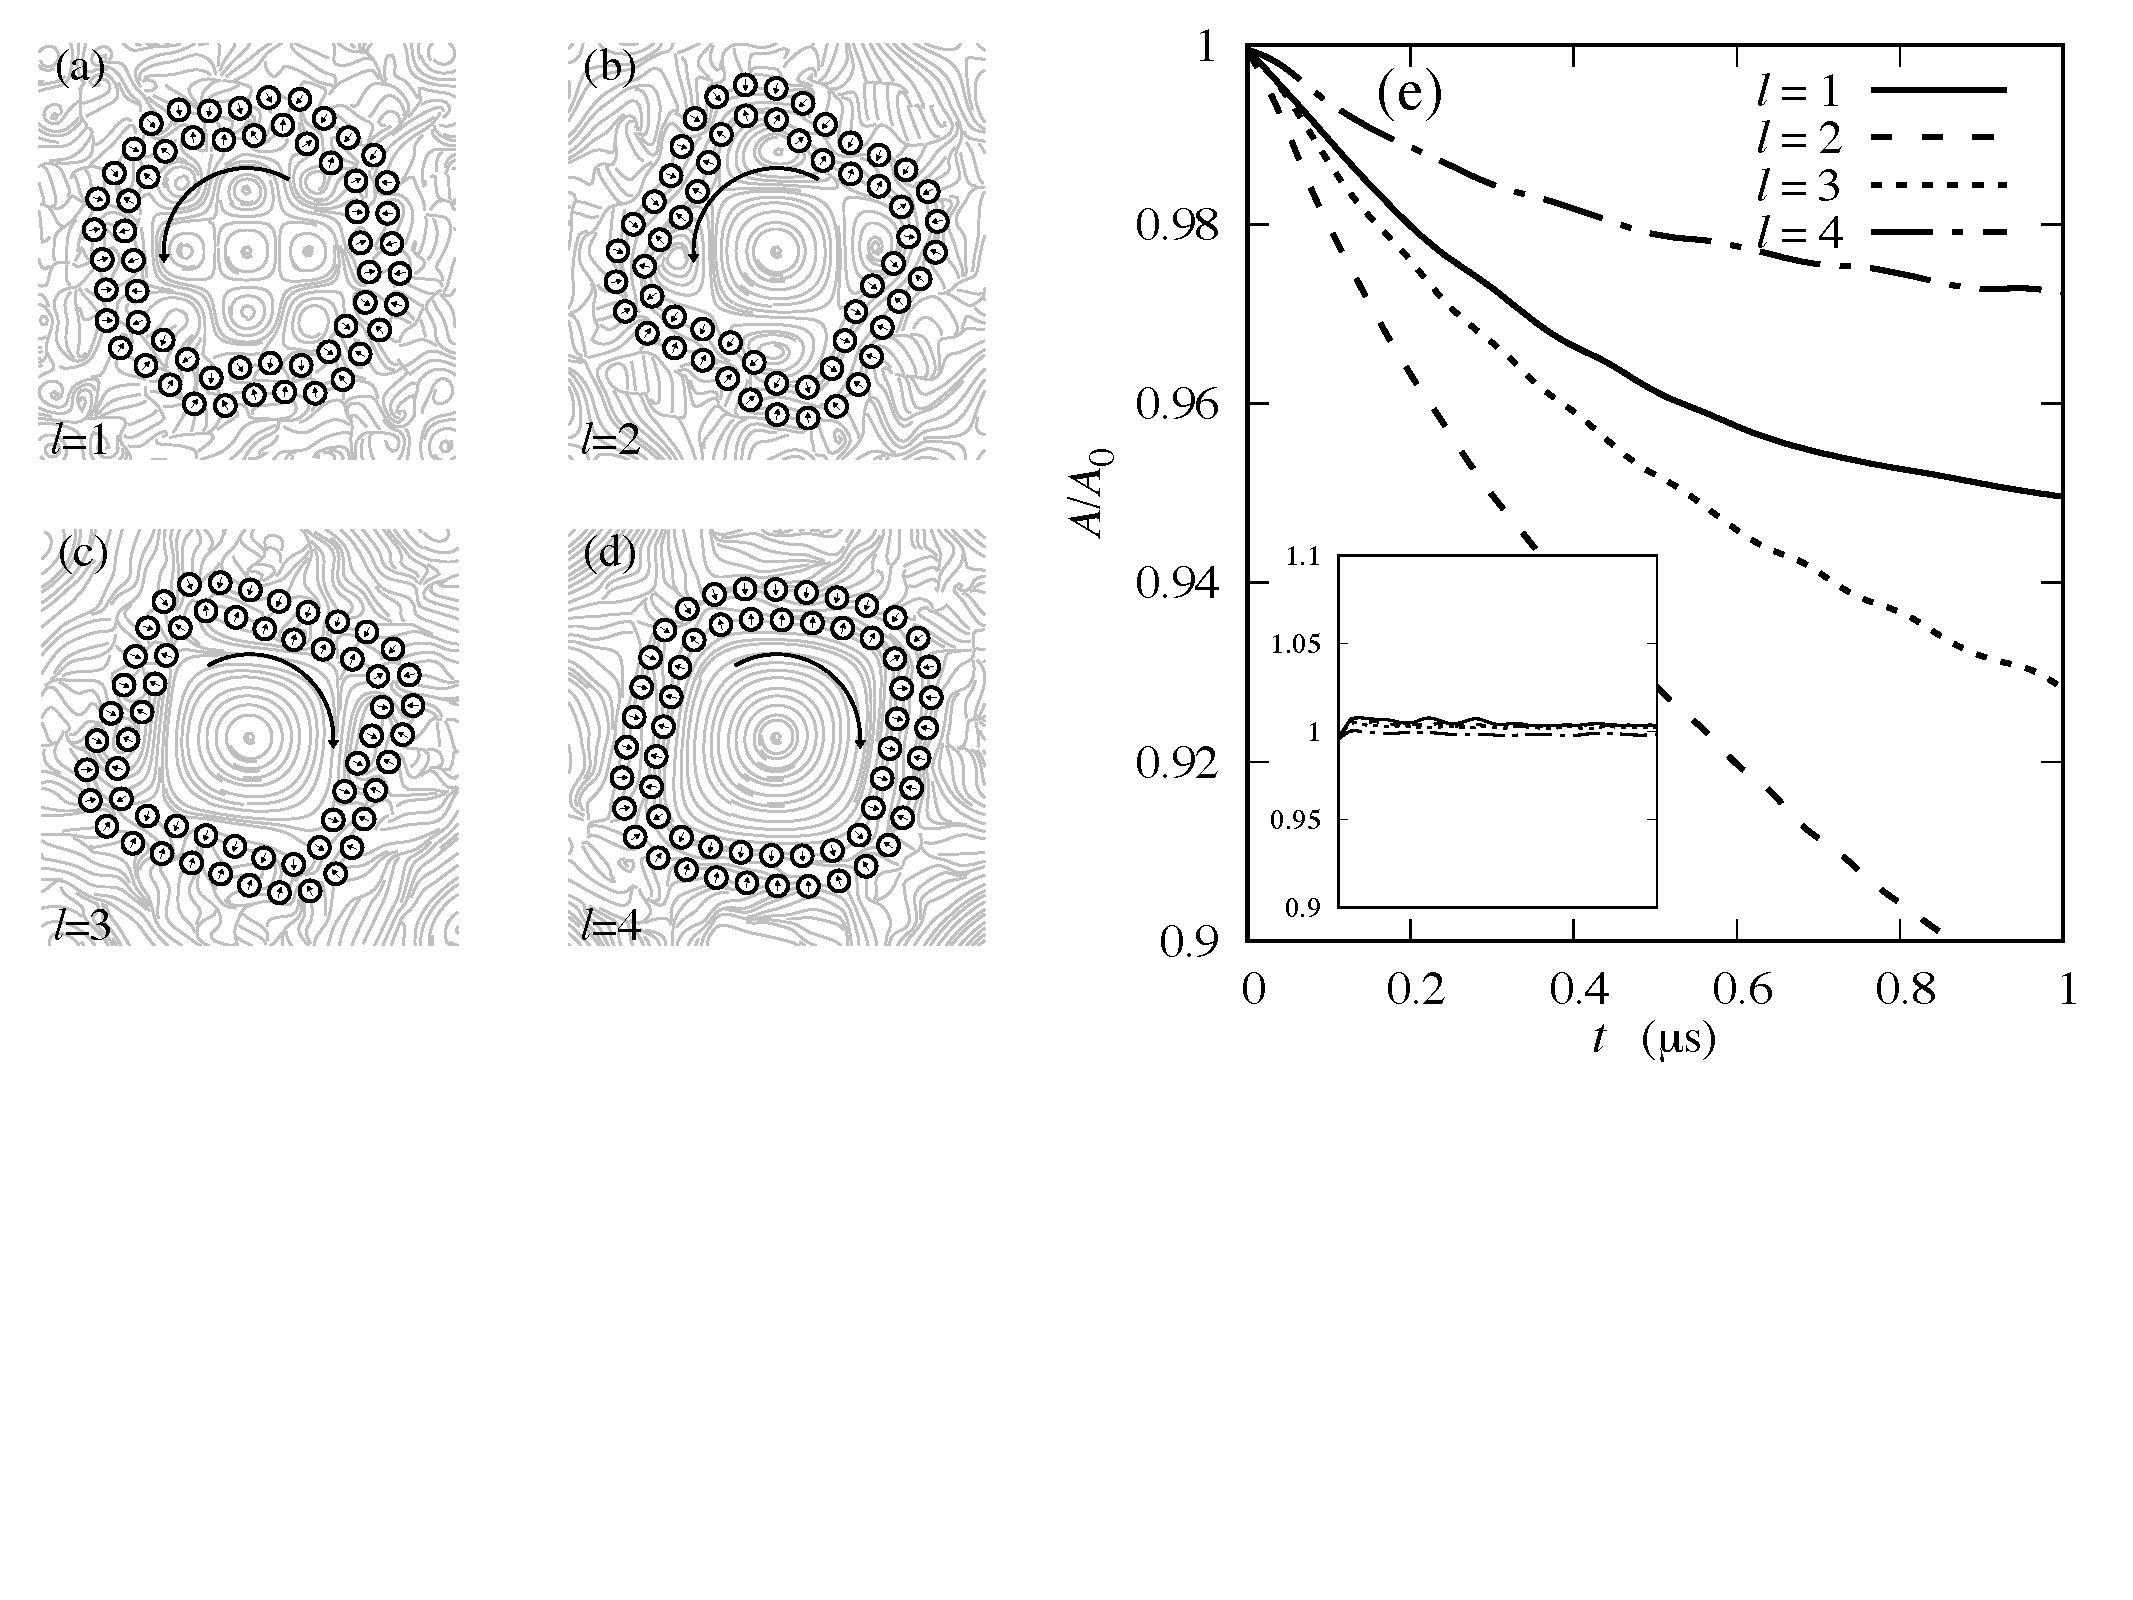
\includegraphics[width=1.0\textwidth]{Figures/Figure7.pdf}
  \end{center}
  \vspace{-20pt}  
  \caption{\label{fig:BTG_Scale} With $V_0=0.1$, panels (a)--(d) show
  the configurations with streamlines of a vesicle is in a TG flow at
  $t=1$ $\upmu$s with $l= 1,2,3,4$, respectively. In panel (e), the
  relative enclosed area $A/A_0$ calculated from the bilayer midplane
  decreases over time. The inset shows the relative length $l/l_0$ which
  remains nearly constant with small magnitude of oscillations. The
  inset and main panel have the same horizontal axis.}
\end{figure}

The vesicle shape is also related to the cell size $l$.
Figure~\ref{fig:BTG_Scale}(a)--(d) show the deformation of a vesicle in
a TG flow for $V_0=0.1$ when $t = 1$ $\upmu$s. For the smallest cell
size $l = 1$ tested, the vesicle is somewhat octagonal and passes
through multiple cells (Figure~\ref{fig:BTG_Scale}(a)). For the largest
cell size $l = 4$, the vesicle is rhomboid and surrounds a single cell. 

In all cases, the JP vesicle tank-treads in TG flow as it does
in the shear flow. The
direction of the tank-treading, however, varies with the cell size
(Figure~\ref{fig:BTG_Scale}(a)--(d), directed arcs). We attribute this
change in rotational orientation to the total rotational moment of the
cells that the vesicle passes through.

We calculate the vesicle area $A$ and length $L$ (initial area $A_0$,
initial length $L_0$) by averaging the area and length of the inner and
outer leaflets. As shown in Figure~\ref{fig:BTG_Scale}(e), the relative
area $A/A_0$ decreases during the simulations, with the rate depending
nonmonotonically on $l$. The relative length $L/L_0$, however, is
constant in $t$ for all cell sizes (Figure~\ref{fig:BTG_Scale}(e),
inset). This implies that the vesicle behaves as an inextensible,
permeable membrane. In previous work, \citet{Fu2022_JFM} determined the
permeability constant of particle-based vesicles in the context of shear
background flow~\cite{chabanon2017, qua-gan-you2021}.



%%%
\begin{figure}
  \begin{center}
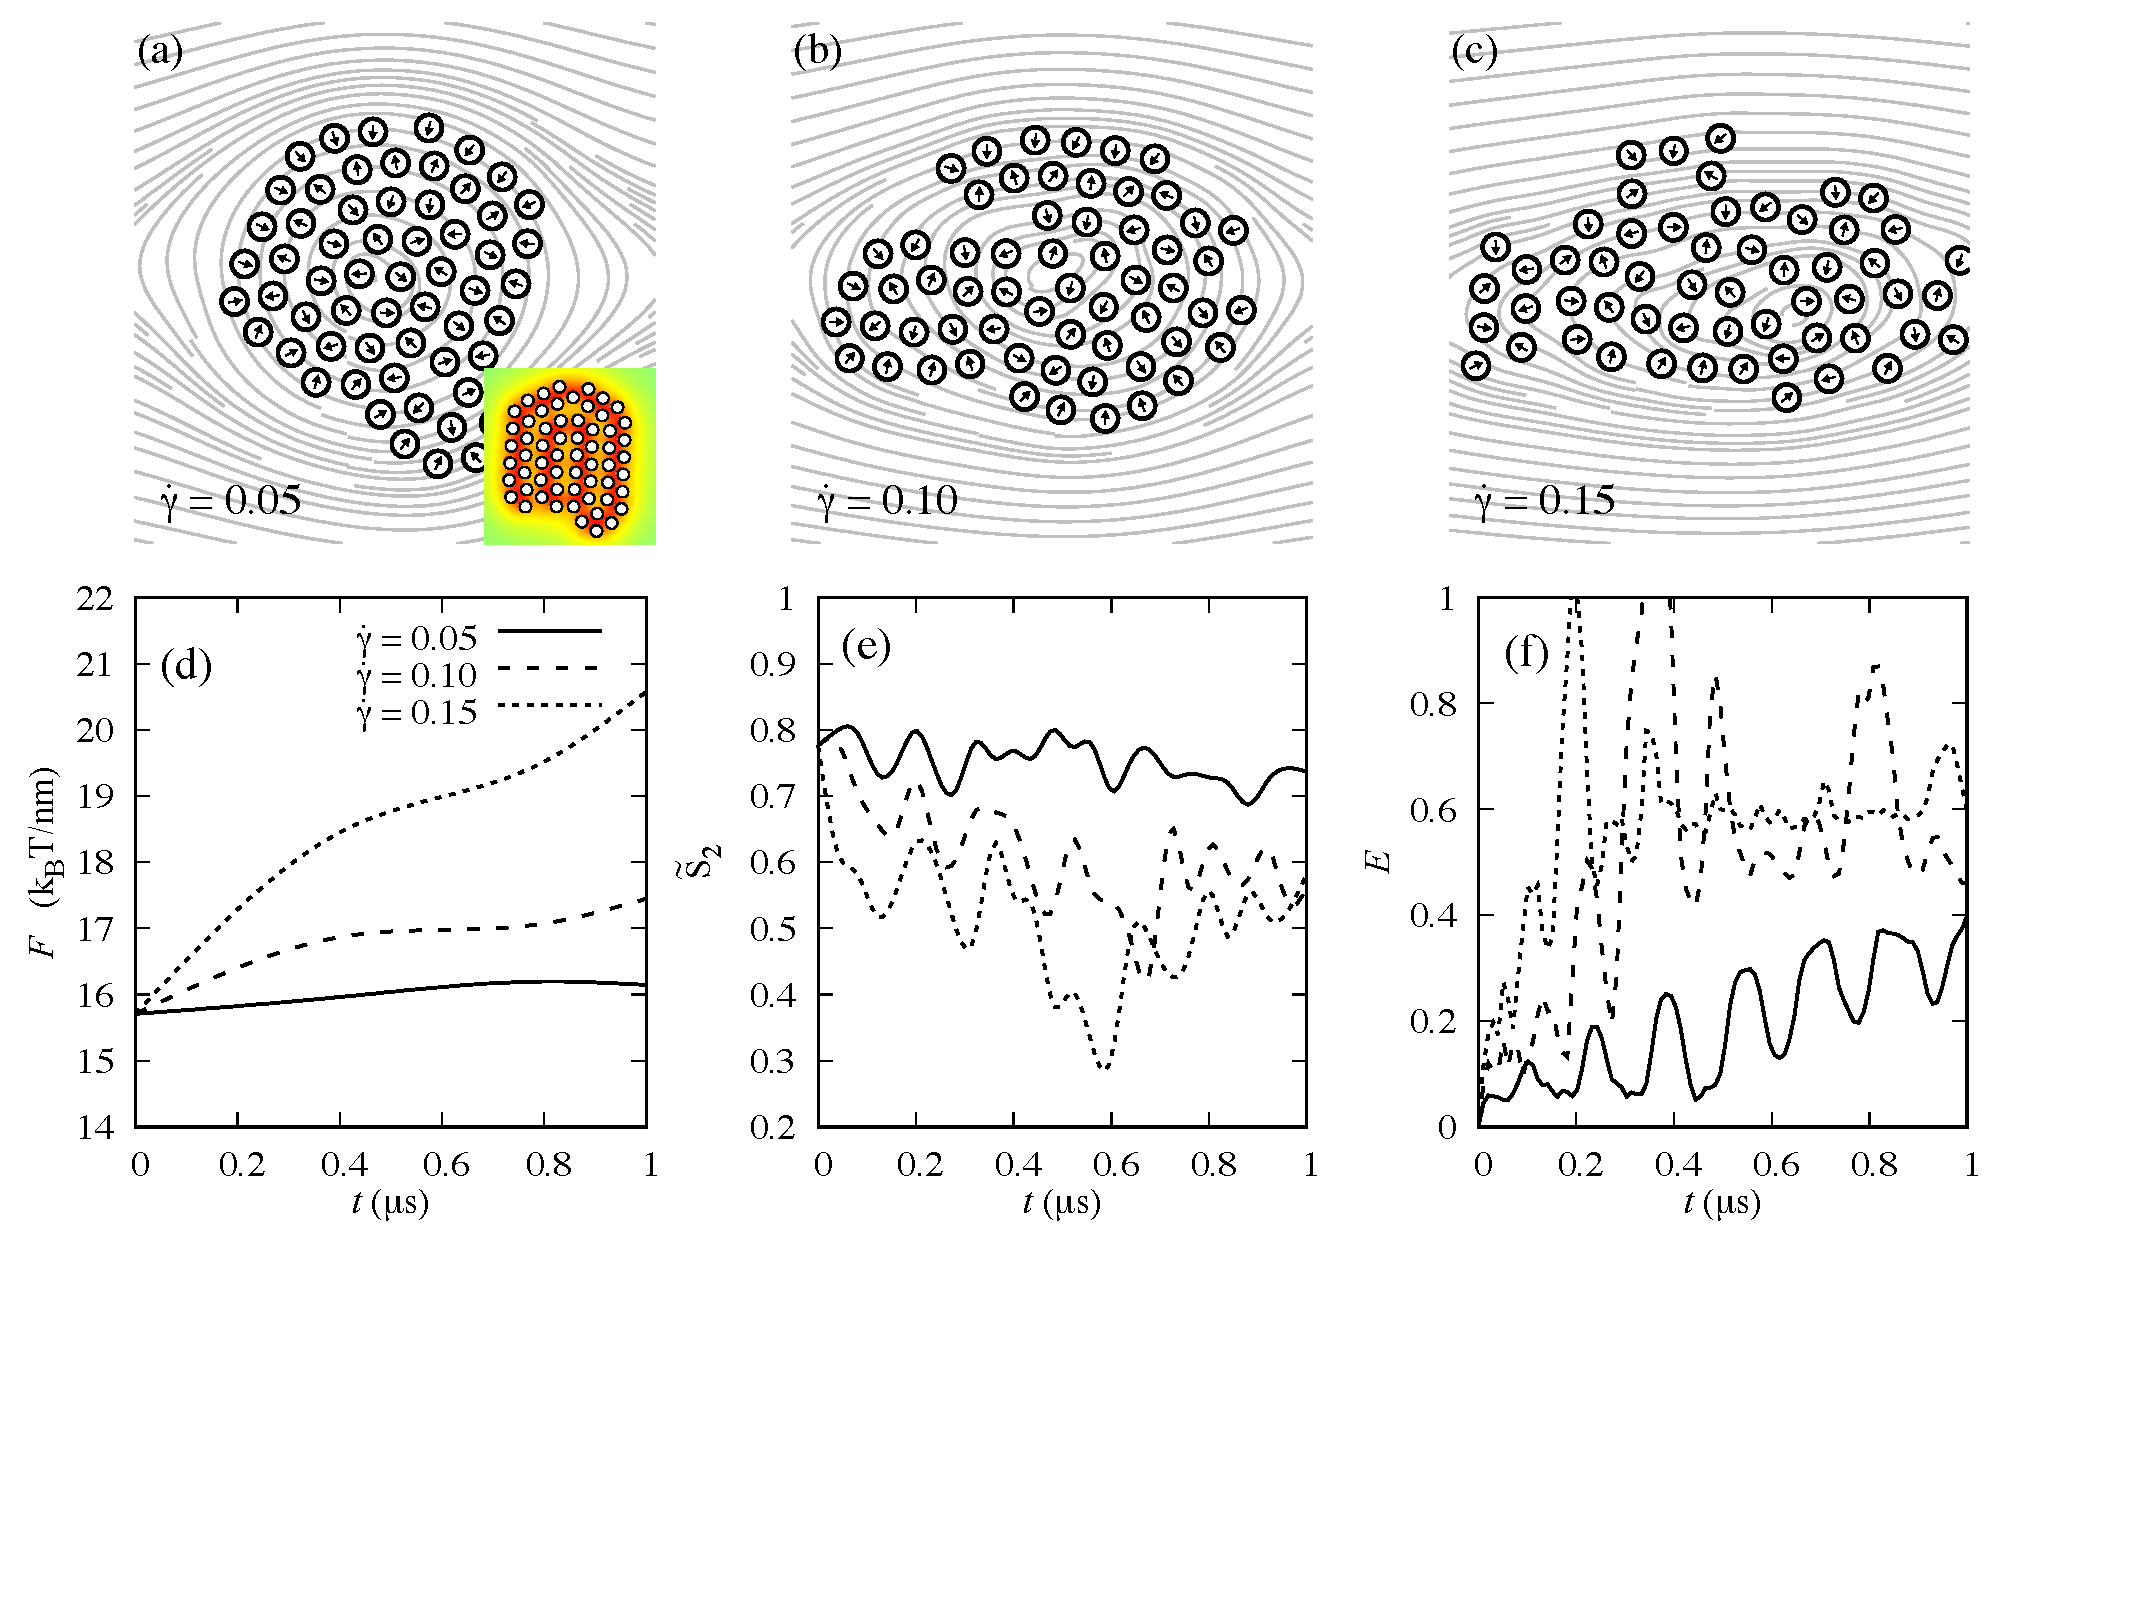
\includegraphics[width=1.0\textwidth]{Figures/Figure8.pdf}
  \end{center}
  \vspace{-20pt}  
  \caption{\label{fig:BC2_shear} A multilamellar structure in a shear
  flow. Panels (a)--(c) are snapshots for $\dot \gamma = \{0.05, 0.1,
  0.15\}$ at $t=0.6\ \upmu$s where the pre-relaxed initial configuration
  is shown in inset of panel (a). The streamlines are plotted in the
  background. Panel (d) shows the free energies; panel (e) shows
  orientational parameter $\tilde{S}_2$; panel (f) shows positional
  parameter E.}
\end{figure}



\subsection{Multilamellar and striated configurations in shear and TG flow}
We have simulated particles for the multilamellar (BC (ii)) and striated
(BC (iii)) boundary conditions, in both shear and TG background flow.
The results are qualitatively similar and will be presented in tandem.
For the multilamellar (BC (ii)) case, we place a 60-particle configuration (inset
of Figure~\ref{fig:BC2_shear}(a)) in shear flow with $\dot\gamma=0.05,
0.1, 0.15$ and in TG flow with $V_0=0.1, 0.15, 0.2$. For the
striated  (BC (iii)) case, we also place a 60-particle configuration (inset of
Figure~\ref{fig:BC3_shear}(a)) in shear and TG background flows. Here,
somewhat larger rates are required to see appreciable deformations for
this boundary condition: $\dot\gamma=0.1, 0.125, 0.15$ and $V_0=0.2,
0.25, 0.3$, respectively.
The BC (ii) and BC (iii) in shear flow cases are visualized in
the latter half of 
Supplementary Movie S2 (low shear rate) and 
Supplementary Movie S4 (high shear rate), respectively.
The low and high flow rates for TG flow are shown in
the latter half of
Supplementary Movie S3 and 
Supplementary Movie S5, respectively. 


In terms of shear flow, the free energies are steady at the lowest shear
rates (Figure~\ref{fig:BC2_shear}(d), Figure~\ref{fig:BC3_shear}(d)).
The free energy of the striated configuration oscillates by $\pm 1$
$\mathrm{k_BT}$/nm due to a square reference region deforming into a
rhomboidal shape under shear flow (Figure~\ref{fig:BC3_shear}(d), solid
curve). No such oscillation is present for the multilamellar
configuration since this shape is circularly isotropic
(Figure~\ref{fig:BC2_shear}(d), solid curve). At the lowest shear rates,
there is, however, oscillation in the strains of both configurations,
while the order parameter $\tilde S_2$ is nearly constant
(Figure~\ref{fig:BC2_shear}(e),(f), Figure~\ref{fig:BC3_shear}(e),(f),
solid curves). In summary, both multilamellar and striated
configurations behave as nearly rigid bodies under shear flow when the
shear rate $\dot \gamma$ is low.

In the high shear rate cases ($\dot\gamma=0.15$), both the multilamellar (BC (ii))
and striated (BC (iii)) configurations become disordered. For BC (ii), the lamella
break apart so that individual bilayers are no longer discernible
(Figure~\ref{fig:BC2_shear}(c)). For BC (iii), the stria peel away from
the main body, but remain individually intact
(Figure~\ref{fig:BC3_shear}(c)). Overall, the particles in BC (ii) and
BC (iii) remain bounded and do not drift away in the shear background
flow like for the BC (i) (Figure~\ref{fig:BC1_shear}(c),
Figure~\ref{fig:Ves_shear}(c)).


\begin{figure}
  \begin{center}
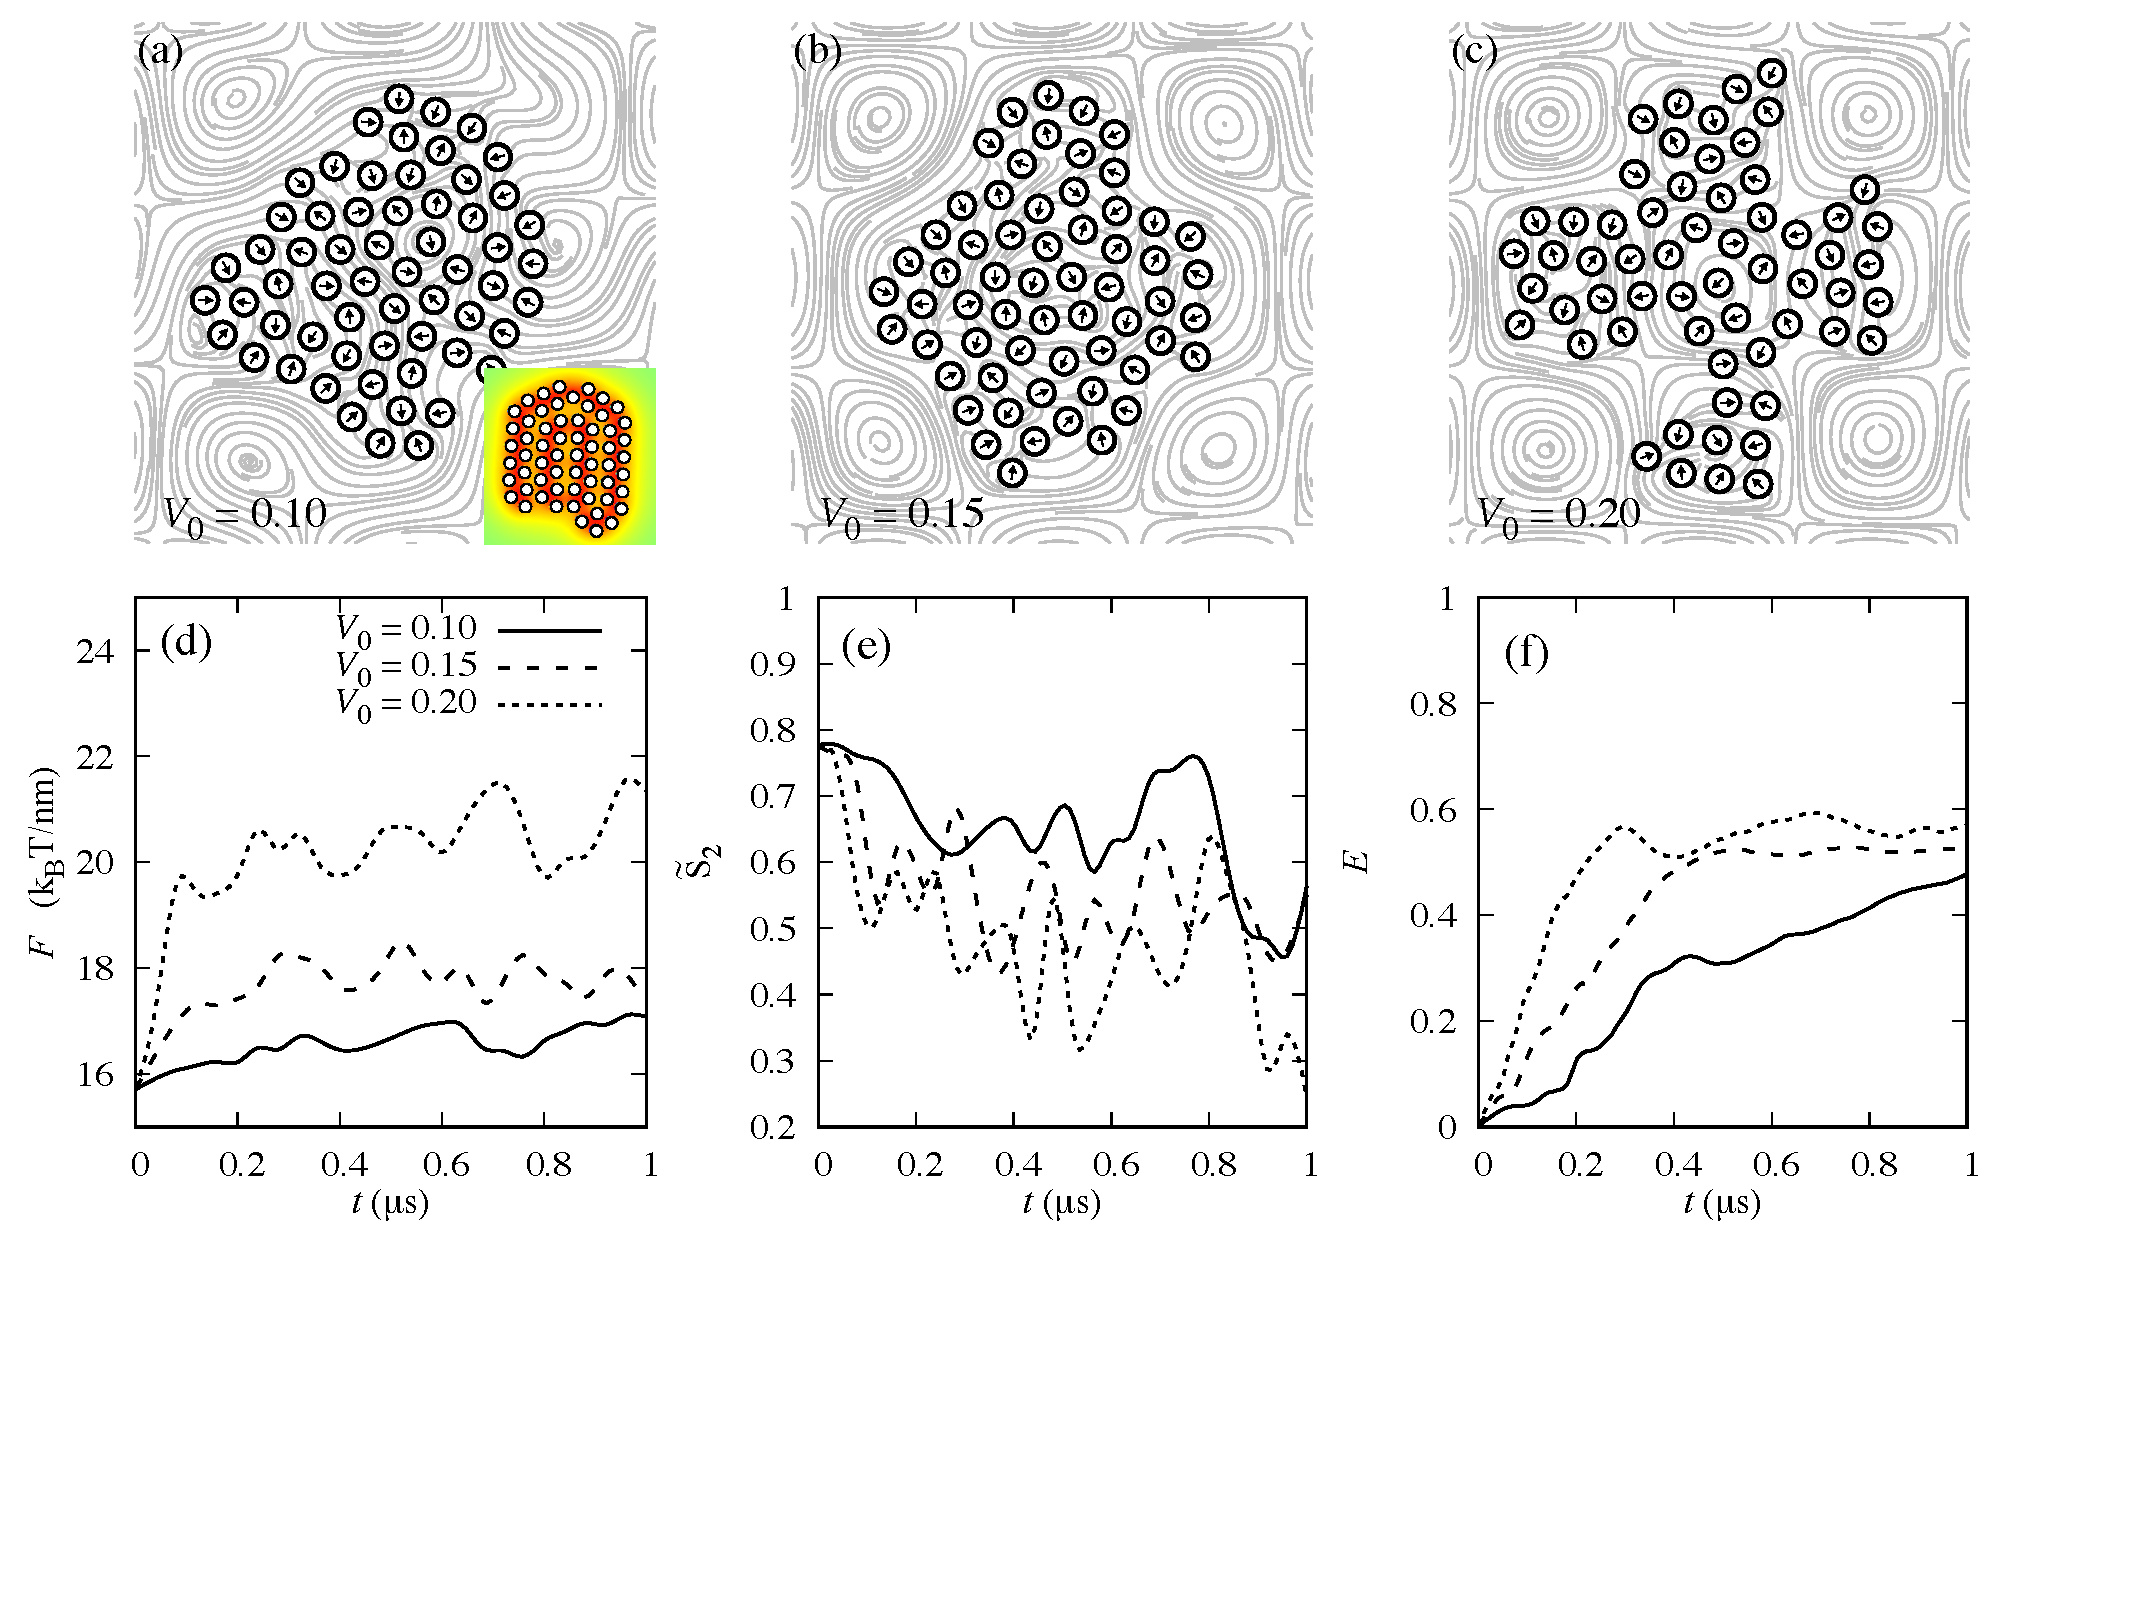
\includegraphics[width=1.0\textwidth]{Figures/Figure9.pdf} 
  \end{center}
  \vspace{-20pt}
  \caption{\label{fig:BC2_TG} A multilamellar structure in a
  Taylor-Green flow. Panels (a)-(c) are snapshots for $V_0 = \{0.1,
  0.15, 0.2\}$ at $t=0.6\ \mu$s where the pre-relaxed initial
  configuration is shown in inset of panel (a). The streamlines are
  plotted in the background. Panel (d) shows the free energies; panel
  (e) shows orientational parameter $\tilde{S}_2$; panel (f) shows
  positional parameter E.}
\end{figure}


Under a TG background flow, the free energy $F$ is also basically
constant for the lowest flow rates $V_0$ (Figure~\ref{fig:BC2_TG}(d),
Figure~\ref{fig:BC3_TG}(d), solid curves). The striated configuration is
unperturbed by the flow, and is engulfed by a single, larger, rotating
flow cell (Figure~\ref{fig:BC3_TG}(a)). The multilamellar configuration
is perturbed by the flow, as seen in the increase in the strain
parameter $E$ (Figure~\ref{fig:BC3_TG}(f), solid curve). The difference
in response to the background flow suggests that the multilamellar
configuration allows for local rearrangement of the particles while
retaining the overall shape.

At large flow rates $V_0$, both configurations depart significantly from
their local equilibrium. The lamella bilayers from BC (ii) break apart,
forming several unlayered bilayer components
(Figure~\ref{fig:BC2_TG}(c)). In BC (iii), the stria also break apart,
but neighboring particles form `X'-like arrangements
(Figure~\ref{fig:BC3_TG}(d)), resembling the doubly alternating director
equilibrium (Figure~\ref{fig:relax}(d), center, top white rectangle).


%%%

\begin{figure}
  \begin{center}
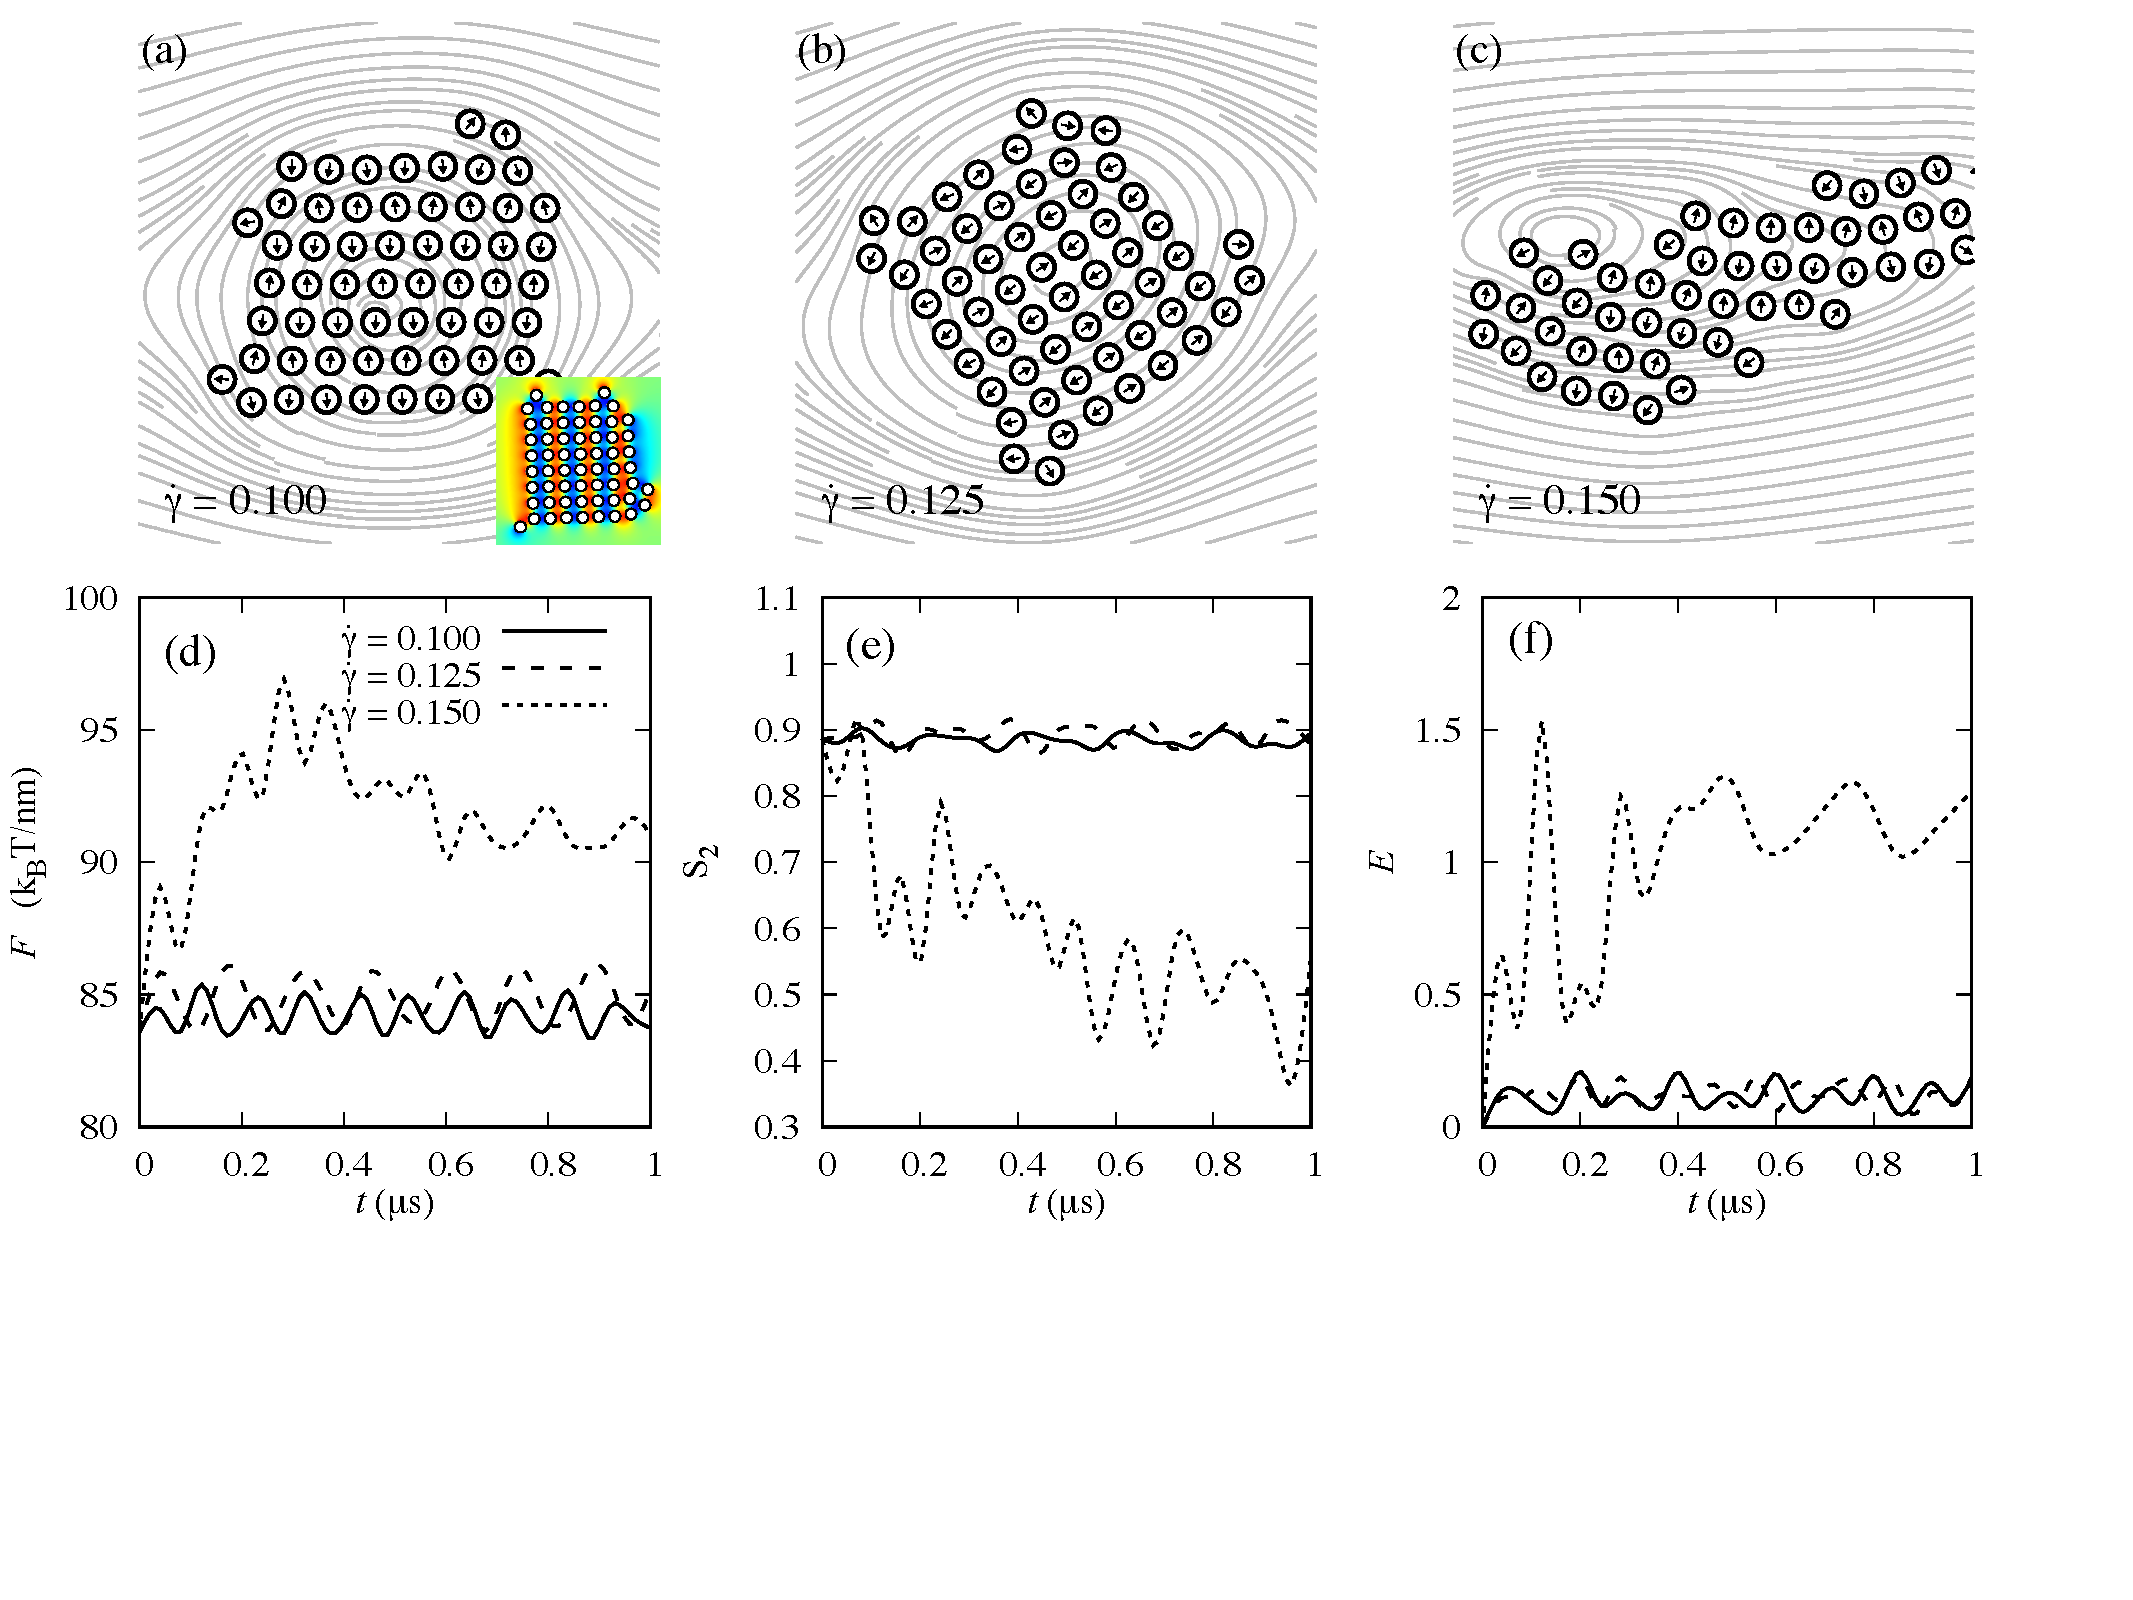
\includegraphics[width=1.0\textwidth]{Figures/Figure10.pdf}        
  \end{center}
  \caption{\label{fig:BC3_shear} A striated configuration in a shear
  flow. Panels (a)-(c) are snapshots for $\dot \gamma = \{0.1, 0.125,
  0.15\}$ at $t=0.1\mu$s where the pre-relaxed initial configuration is
  shown in inset of panel (a). The streamlines are plotted in the
  background. Panel (d) shows the free energies; panel (e) shows
  orientational parameter $\tilde{S}_2$; panel (f) shows positional
  parameter E.}
\end{figure}


\begin{figure}
  \begin{center}
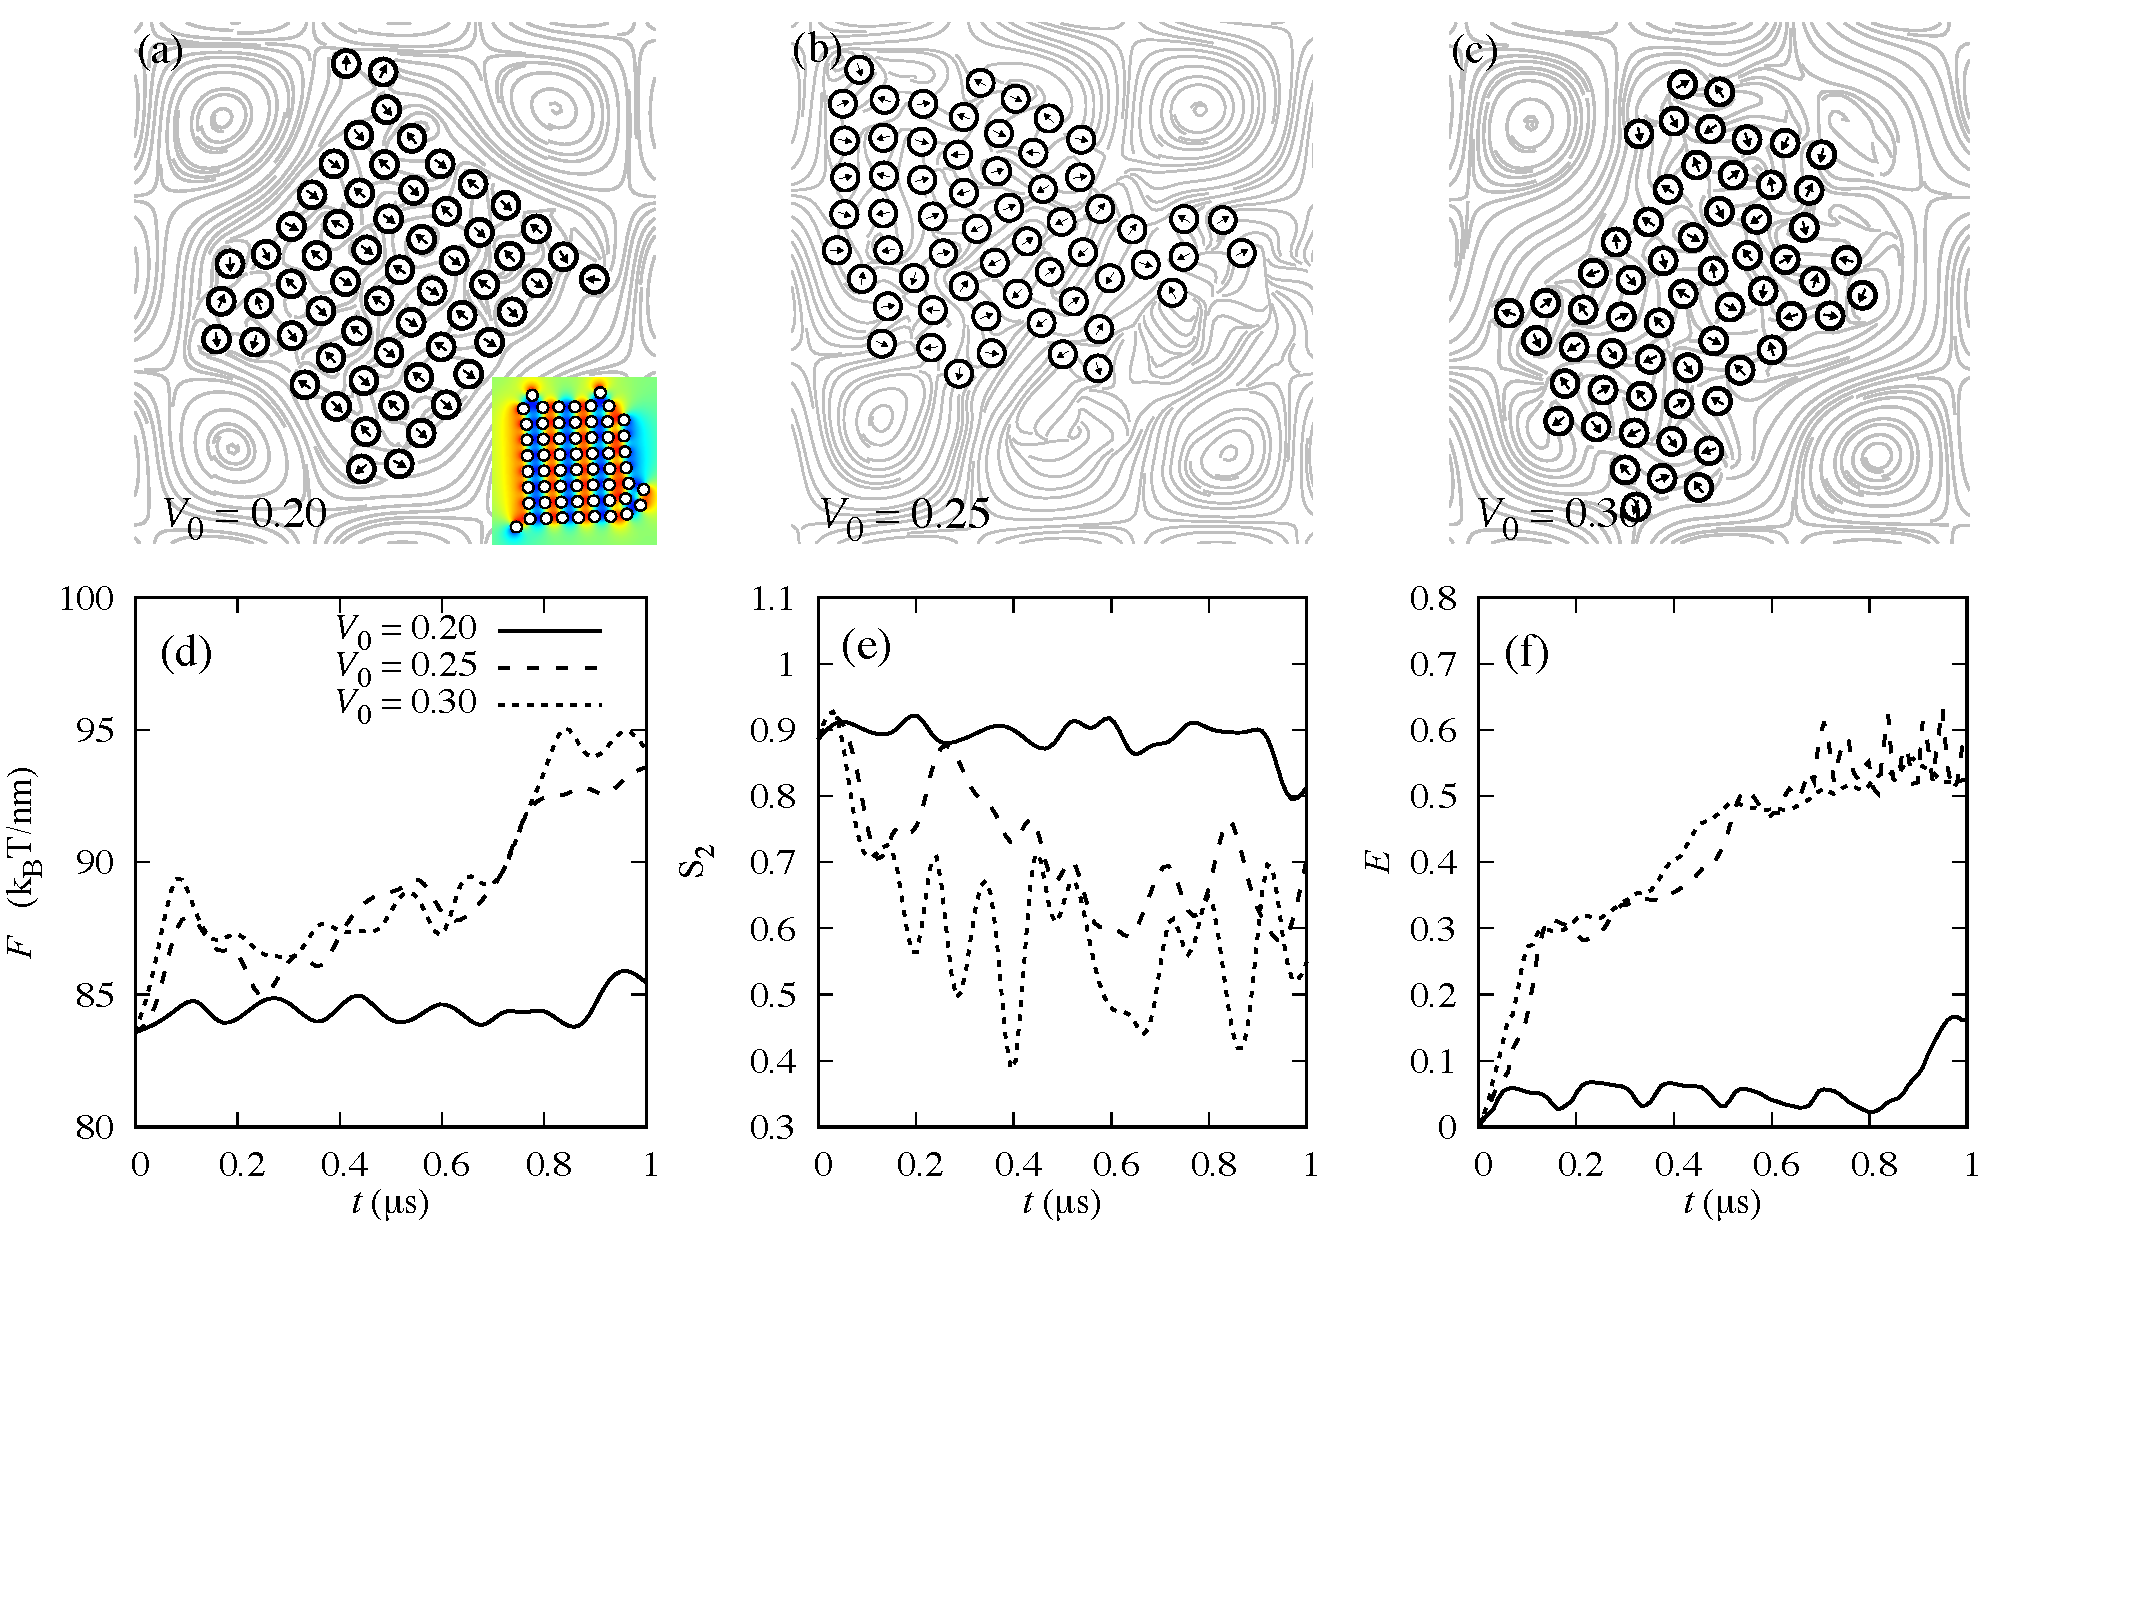
\includegraphics[width=1.0\textwidth]{Figures/Figure11.pdf}            
  \end{center}
  \vspace{-20pt}  
  \caption{\label{fig:BC3_TG} A striated configuration in a Taylor-Green
  flow. Panels (a)-(c) are snapshots for $V_0=\{0.2, 0.25, 0.3\}$ at
  $t=0.4\mu$s where the pre-relaxed initial configuration is shown in
  inset of panel (a). The streamlines are plotted in the background.
  Panel (d) shows the free energies; panel (e) shows orientational
  parameter $\tilde{S}_2$; panel (f) shows positional parameter E.}
\end{figure}



\section{Discussion\label{sec:discussion}}
Results in \S~\ref{sec:results} are from simulations with $N_b = 60$ particles.
%Our results were for $N_b = 60$ particles. 
This particle number was
large enough for the JP to form measurable structures while giving
manageable simulation times (days) on a single computing processor. The
simulation time for $N_b = 198$ in Figure~\ref{fig:relax} and
Figure~\ref{fig:relax_energy} was several weeks, and so we avoided
simulations of this size for our results. We used $N = 16$ grid points
per particle for all simulations. We performed a convergence study and
found that using $N = 16$ or $N = 24$ grid points per particle gave
quantitatively indistinguishable results. The time courses consisted of
$O(10^3)$ time steps with $\Delta t = 0.2$ ns.

The free energy $F$ defined in~\eqref{eq:free_energy} scales with the
boundary data $g$ and repulsion modulus $M$. 
%To remove the degree of freedom in the boundary data, 
We thus scale all boundary data so that the
square integral of $g$ is independent of the type of boundary condition; BC
(i), (ii), or (iii). This way, for a fixed configuration, the
hydrophobic interaction portion of the free energy (the integral
in~\eqref{eq:free_energy}) converges to $\gamma N_b$ in the limit
$\rho = 0$. This gives a free energy per particle that is independent of
the shape and intensity of the hydrophobic interface. In practice, $\rho
> 0$ is fixed and the JPs assume different configurations. As a result,
the equilibrium energies per particle in our simulations are different
and depend on the boundary condition (Figure~\ref{fig:relax_energy}).
They are about 0.26 $\mathrm{k_BT}$/nm for BC (ii), 0.55
$\mathrm{k_BT}$/nm for BC (i), and 1.4 $\mathrm{k_BT}$/nm for BC (iii).

Next, we impose a flow on the JP suspension to study
deformations of JP assemblies as a function of flow strength. There are three categories
of boundary conditions---BC (i), BC (ii), and BC (iii)---that form
bilayer, multilamellar, and striated configurations, respectively. For
BC (i), we consider both an unstructured bilayer and a vesicle
bilayer. The background flows are a linear shear flow and a steady TG flow.

We characterize the effective material properties of the JP
structures based on the changes in free energy, orientational order, and
strain as a function of flow strength. Generally, $F$ increases, $\tilde
S_2$ decreases, and $E$ increases with increases in both $\dot \gamma$
and $V_0$, as expected. Structurally, the striated JP configuration for
BC (iii) behaves the most like a rigid body over the flow strengths
tested. For this structure, the deformation measures are constant in
time for shear rates $\dot \gamma$ up to $0.15$ and TG flow rate $V_0$
up to $0.25$ (Figure~\ref{fig:BC3_shear} and Figure~\ref{fig:BC3_TG}).
In contrast, a $25\%$--$50 \%$ smaller value for $\dot \gamma$ or $V_0$ is
required to observe nonrigid deformations for the BC (i) and BC (ii)
cases.

In terms of fluid behavior, the multilamellar (BC (ii)) structure
behaves as a shear thinning fluid while the striated structure (BC (iii))
has a finite yield stress. Qualitatively, the strains for BC (ii)
increases gradually with shear rate (Figure~\ref{fig:BC2_shear}(f)). In
contrast, the strains for BC (iii) are constant over a range of flow
strengths and then increase when the flow strengths are large enough to
deform the body (Figure~\ref{fig:BC3_shear}(f)). To quantify this
behavior, we form 
\begin{align}
\label{eq:mu_asm}
\mu_{\text{asm}} = \frac{\dot \gamma}{\dot E} \mu 
\end{align}
as an effective dynamic viscosity of the particle assemblies. The
numerator $\dot \gamma \mu$ gives the force per area provided by the
solvent stresses where $\mu = 1$ mPa s is the solvent viscosity. The
strain rate $\dot E$ of the body is the slope of a linear fit to the
strain curves e.g., in Figure~\ref{fig:BC2_shear}(f).


%%%


\begin{figure}[t]
\begin{center}
  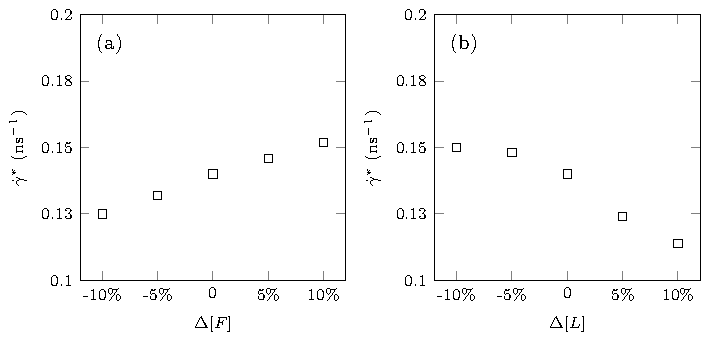
\includegraphics[height=0.3\textheight]{ChangeLengthForce.pdf}
\end{center}
\begin{caption}{\label{fig:PramChange}
When the force parameters are tuned in the same percentage change, a linear proportional relationship between changes (square symbol) and the critical shear rates $\dot\gamma^*$ is shown in numerical results. The same adjustment in length parameters give a nearly linear trend with an inverse proportional relationship between changes (triangle symbol) and the critical shear rates.}
\end{caption}
\end{figure}

To further examine the contest between shear and head-tail attraction, we found that a 5\% and 10\% relative increases in the parameters $\gamma$ and
$M$ resulted in 4.29\% and 8.57\% relative increases in critial shear rate $\dot\gamma$, from 0.14 to 0.146 and 0.14 to 0.152, respectively. 
A proportional relationship is observed as the parameters decrease and it is shown in Figure~\ref{fig:PramChange}.
Moreover, Figure~\ref{fig:PramChange} also shows that 5\% and 10\% decreases in the particle radius c, screening length $\rho$ and repulsion distance $\rho_0$ gave 5.71\%  and 7.14\% increase in $\dot\gamma$ from 0.14 to 0.148 and 0.14 to 0.15.
In addition, 5\% and 10\% increases in length parameters gave 11.43\% and 18.57\% decrease in critical shear rate $\dot\gamma$.
The overall result provides another evidence that a different hydrophobicity suggests a dissimilar rheology and dynamics viscosity from the suspended vesicle experiments.

%%%


The viscosities of particle assemblies calculated from \eqref{eq:mu_asm} are shown in
Table~\ref{tbl:bcii_visc}. The middle row gives the solid area fraction
$\phi$; the sum of the rigid particle areas divided by the total area of
the solvent and particle region. We observe that for the multilamellar
structure, $\mu_{\text{asm}}$ decreases with increasing shear rate. The
predicted viscosities of the particle assemblies are on the order of
hundreds of times that of water, consistent with suspension viscosities
for noninteracting particles~\cite{KONIJN201461}. In the case of
striated structures, viscosity is effectively infinite for the lower two
of the shear rates, and then drops to a finite value $\mu_{\text{asm}} =
60$ mPa s when the shear rate reaches $0.15$ ns$^{-1}$.
\begin{table}
  \caption{\label{tbl:bcii_visc} The dynamic viscosity of assemblies
  $\mu_{\text{asm}}$ (mPa s).}
\centering
\begin{tabularx}{0.7\textwidth}{c|X|X|X||X|X|X}
&\multicolumn{3}{c||}{BC (ii)} & \multicolumn{3}{c}{BC (iii)}\\
\hline
  $\dot \gamma$ & 0.05 & 0.10 \quad & 0.15 & 0.100 & 0.125 & 0.15\\
  \hline
  $\phi$ & 0.50 & 0.47 & 0.41 & 0.47 & 0.46 & 0.45 \\
  \hline
  $\mu_{\text{sus}} $ & 401 & 66 & 42 & 2.5e3 & 1.4e3 & 60\\
\hline
\end{tabularx}
\end{table}

In the case of BC (i), our previous work~\cite{Fu2022_JFM} calculated a
friction coefficient $b$ for the intermonolayer slip between the two
leaflets of a bilayer. \citet{denOtter2007,Zgorski2019} and
\citet{doi:10.1073/pnas.2100156118} have calculated in-plane viscosities
for fully three-dimensional bilayers. Although not part of this work, it
is in principle possible to obtain an in-plane viscosity using the
hydrophobic potential~\eqref{eq:free_energy} by replacing the boundary
condition~\eqref{eq:bc-type} with one that is everywhere constant, in
effect modeling lipids in a bilayer as an array of elongated, purely
hydrophobic pillars. 

While increased flow strengths generally injected energy into the
suspension, the simulation results show that the unstructured bilayer
actually increases orientational order and has somewhat lower free
energy under low shear rates (Figure~\ref{fig:BC1_shear}(d,f)). This
effect suggests that in amphiphilic suspensions, it might be possible to
decrease the excess area of the system by subjecting the suspension to a
moderate shear flow (Supplementary Movie S2, right panel).
Not all background flows produce this
``organizing'' effect, as it is not observed in the TG background flow
case (Figure~\ref{fig:BC1_TG}, Supplementary Movie S3, right panel).
\citet{PhysRevLett.128.256102} have
shown how to drive particle clusters into arbitrary target shapes by
solving a first passage problem.

The characteristics of the self-assembly of amphiphilic JP into
onion-like dendrimersomes like for BC (ii) were previously studied by molecular dynamics
simulations~\cite{C9NR05885K}. The molecular dynamics simulations use an
anisotropic pair potential to describe the particle interactions
where a harmonic form describes the repulsive part and an anisotropic
attractive part describes the hydrophobic interactions~\cite{HongCacciutoLuijtenGranick2008}.
We also use a pair potential $P$ in the free energy \eqref{eq:free_energy} for repulsion,
whereas the long-range, hydrophobic attraction \eqref{eq:FandTdef}
is nonadditive and comes from domain-dependent variation of
the water order parameter $u(\xx)$ in the bulk.


\citet{kohl-cor-che-vee22} have simulated JP suspensions in three
dimensions using the same free energy formulation of hydrophobic
attraction used in the present work. They observed spontaneous
aggregation into micelles generically and formation of bilayers when the
initial configuration was chosen sufficiently close to the final
configuration. They also studied self-assembly of bipolar electric JP,
which corresponds to our BC (iii) JP (but electric potential, instead of a water order parameter),
to define the interaction.  Due to the differing interaction,
bipolar electric particles form parallel chains that
repel. In contrast, the hydrophobic interaction between stria is
attractive. The existence of 'X'-shaped local arrangements as a local
equilibrium (Figure~\ref{fig:relax}(d), top, middle rectangle) further
suggests there may be greater diversity in the set of possible
equilibria in three-dimensions when employing hydrophobic attraction.